\documentclass[a4paper,12pt,openany,oneside,utf-8]{ctexbook}
%\documentclass[a4paper,12pt,openany,oneside,utf-8]{cctbook}
%\usepackage{hyperref}
%\hypersetup{CJKbookmarks=true}
\usepackage{amssymb,amsmath}
\usepackage{subcaption}
\usepackage[amsmath,thmmarks]{ntheorem}
\usepackage{fancyhdr}
\usepackage{graphicx}
\usepackage{titletoc}%????,
\usepackage{epsfig,picins,picinpar}
\usepackage{setspace}
%\usepackage[top=2.54cm,bottom=2.54cm,left=2.54cm,right=2.54cm]{geometry}
\usepackage{geometry}
\geometry{left=3.0cm,right=2.0cm,top=2.5cm,bottom=2.5cm,}
\usepackage{amsmath}
\usepackage{mathtools} % offer \coloneqq to show := [see https://tex.stackexchange.com/questions/194344/symbol-for-definition]
%%%%%%%%%%%%%%%%%%%%%%%%new
\usepackage[super,square,comma,sort&compress]{natbib}
\usepackage{multirow}
\usepackage{dsfont}
\usepackage{booktabs}
\usepackage{epstopdf}
\usepackage{ccmap}
\bibliographystyle{gbt7714-2015}%{elsarticle-num}%{elsarticle-num}%{plain}%{elsarticle-num-names}%




%%%%%%%%%%%%%%%%%%%%%%??????
%\usepackage{natbib}     % adding a package for \citet{}, \citep{}, \citet*{}, \citep*{}
\usepackage{amssymb} %% The amssymb package provides various useful mathematical symbols
\usepackage{amsmath}
\DeclareMathOperator*{\argmax}{arg\,max}
\usepackage{bm}         % adding a package for \bm{\widehat{\beta}}
\usepackage{makecell}   % makecell, see: https://blog.csdn.net/cy_tec/article/details/51436434
\usepackage{multirow}   % Latex Table, see: https://blog.csdn.net/canhui_wang/article/details/72920963
\usepackage{booktabs}   % for \cmidrule, see: https://zhidao.baidu.com/question/306414034088577164.html
\usepackage{graphicx}   % adding a package for loading figures
\usepackage{threeparttable}   % adding a package for tablenotes
\usepackage{algorithm}
\usepackage{algorithmicx}
\usepackage{algpseudocode}
\usepackage{titlesec}    % for \titleformat
\usepackage{indentfirst}   % ??????????????????????\usepackage{indentfirst}?????? see: https://zhidao.baidu.com/question/207438548.html
\usepackage{caption}   % for \captionsetup, see: https://blog.csdn.net/kebu12345678/article/details/76957377?locationNum=9&fps=1
\usepackage{makecell}  % for \Xcline  \Xhline, see: http://blog.sina.com.cn/s/blog_5e16f1770100mvtd.html
\floatname{algorithm}{Algorithm}  % Ref: https://blog.csdn.net/lwb102063/article/details/53046265
\renewcommand{\algorithmicrequire}{\textbf{Input:}}
\renewcommand{\algorithmicensure}{\textbf{Output:}}
\usepackage{paralist} % for \begin{enumerate}, see: http://bbs.ctex.org/forum.php?mod=viewthread&tid=62084
\usepackage{times}
\usepackage{mathptmx}
%%%%%%%%%%%%%%%%%%%%%%??????



%%%%%%%%%%%%%%%%%%%%%%%%
%\renewcommand\sectionname{\arabic{section}}
%\renewcommand\sectionformat{\centering}
%\renewcommand\subsectionname{\arabic{section}.\arabic{subsection}}
%\renewcommand\subsectionformat{}
%\renewcommand\subsubsectionname{\arabic{section}.\arabic{subsection}.\arabic{subsubsection}}
%\renewcommand\subsubsectionformat{}

\allowdisplaybreaks[4]
\renewcommand{\baselinestretch}{1.5}
%\renewcommand{\chaptername}{{Chapter\thechapter}}
\renewcommand{\chaptername}{?{\thechapter}?}
\renewcommand\bibname{????}
\renewcommand\contentsname{??}
%\renewcommand{\sectionname}{{\thechapter}.\arabic{section}}

\renewcommand {\thetable} {\thechapter{}.\arabic{table}}
\renewcommand {\thefigure} {\thechapter{}.\arabic{figure}}
\renewcommand {\theequation} {\thechapter{}-\arabic{equation}}

% ??????
\newcommand{\chuhao}{\fontsize{48pt}{\baselineskip}\selectfont}
\newcommand{\xiaochuhao}{\fontsize{36pt}{\baselineskip}\selectfont}
\newcommand{\yihao}{\fontsize{28pt}{\baselineskip}\selectfont}
\newcommand{\xiaoyihao}{\fontsize{25pt}{\baselineskip}\selectfont}
\newcommand{\erhao}{\fontsize{21pt}{\baselineskip}\selectfont}
\newcommand{\xiaoerhao}{\fontsize{17pt}{\baselineskip}\selectfont}
\newcommand{\sanhao}{\fontsize{15.75pt}{\baselineskip}\selectfont}
\newcommand{\xiaosanhao}{\fontsize{15pt}{\baselineskip}\selectfont}
\newcommand{\sihao}{\fontsize{13pt}{\baselineskip}\selectfont}
\newcommand{\xiaosihao}{\fontsize{12pt}{\baselineskip}\selectfont}
\newcommand{\wuhao}{\fontsize{10.5pt}{\baselineskip}\selectfont}
\newcommand{\xiaowuhao}{\fontsize{9pt}{\baselineskip}\selectfont}
\newcommand{\liuhao}{\fontsize{7.875pt}{\baselineskip}\selectfont}
\newcommand{\qihao}{\fontsize{5.25pt}{\baselineskip}\selectfont}%\newcommand\kaishu{\CJKfamily{kai}}


\CTEXsetup[name={?,?}, number=\arabic{chapter}]{chapter}
\titleformat{\chapter}{\centering\sanhao\bfseries}{?\,\thechapter\,?}{1em}{}
\titlespacing*{\chapter} {0pt}{-10.5pt}{12pt}

\titleformat{\section}{\xiaosanhao\bfseries}{\thesection}{1em}{}
\titlespacing*{\section} {0pt}{12pt}{12pt}

\titleformat{\subsection}{\sihao\bfseries}{\thesubsection}{1em}{}
\titlespacing*{\subsection} {0pt}{0pt}{5.25pt}

\DeclareCaptionFont{fivehao}{\fontsize{10.5pt}{11pt}\selectfont #1}
\pagestyle{fancy}%
\renewcommand{\headrulewidth}{0pt}
\renewcommand{\footrulewidth}{0pt}
\addtolength{\headheight}{0\baselineskip}
\addtolength{\headwidth}{0\marginparsep}
\addtolength{\headwidth}{0\marginparwidth}
\setlength{\headsep}{5mm}%
\fancyhf{}


\begin{document}
	\theoremstyle{plain} \theoremseparator{}
	\theoremindent0cm\theoremnumbering{arabic} \theoremsymbol{}
	
	
	\fancypagestyle{plain}{%
		\fancyhead{}
		\fancyhead[CE,CO]{\xiaowuhao{}}}
	%\begin{titlepage}
	%\fancypagestyle{plain}{\pagestyle{fancy}}
	%\fancyhead[C]{\xiaowuhao}
	%\vskip 4mm
	%\xiaowuhao ????? \hspace{9cm}??????O212.1
	%
	%\vskip 6mm
	%
	%\begin{figure}[htbp]
	%\centering
	%
\includegraphics[width=140mm,height=22mm]{zjgsu.jpg}
	%\end{figure}
	%
	%\vskip 10mm
	%
	%\begin{spacing}{1.0}
	%\begin{center}
	%\chuhao\textbf{??????}
	%\end{center}
	%
	%\vskip 20mm
	%\begin{center}
	%\hspace{0.01mm}\sanhao\textbf{?????\underline{??SM-?????ARMA????}}
	%\end{center}
	%\end{spacing}
	%\vspace{24mm}
	%
	%\begin{center}
	%\textbf{\kaishu\sanhao ?????\underline{\quad \quad \quad \quad \quad  ?? \quad \quad \quad \quad}}
	%\end{center}
	%
	%
	%\begin{center}
	%\textbf{\kaishu\sanhao ?????\underline{\quad \quad \quad \quad \ ??? \quad \quad \quad \quad}}
	%\end{center}
	%
	%
	%\begin{center}
	%\textbf{\kaishu\sanhao ?????\underline{\quad \quad  \quad ?????? \  \quad \quad}}
	%\end{center}
	%
	%\begin{center}
	%\textbf{\kaishu\sanhao ?????\underline{\quad \quad \quad \quad \ ??? \quad \quad \quad \quad }}
	%\end{center}
	%
	%\
	%
	%\
	%
	%\
	%
	%
	%\begin{center}
	%\kaishu\sanhao ?????2019 ?10?
	%\end{center}
	%
	%\end{titlepage}
	
	
	\frontmatter
	\pagenumbering{Roman}
	\cfoot{\thepage}
	\newpage
	\begin{center}
		\heiti\sanhao\textbf{?\quad ?}
	\end{center}
	\hspace*{\fill} \\ %???
	\begin{spacing}{1.5}
		{\xiaosihao\songti ???????????????????????????????????????????????????????????ARMA?????????????????????????????????}
	\end{spacing}
	\begin{spacing}{1.5}
		{\xiaosihao\songti ???????ARMA???????????????????(ML)???????(LS)?????ML???LS???????????????????????????????????????????????????????????????????ML???LS????????????????????????(LAD) ??M-?????ML???LS?????LAD???M-???????????ML???LS?????M-????????????????????????????????????????????????????????????????????????????????????}
	\end{spacing}
	\begin{spacing}{1.5}
		{\xiaosihao\songti ?????????????????M-???????????????????????????ARMA???SM-???SM-?????????????????????????????????????????????????????????????????????????????????????SM-????????????????????ARMA?????????????????????????SM-??????????????????????ARMA????????ARMA?????????????????????????????????????????SM-???LS???LAD ??????????SM-???MSE??????????SM-???????????????????????SM-???MAE?MSE???LS???LAD ???}
	\end{spacing}
	\hspace*{\fill} \\ %???
	\noindent {\xiaosihao\songti \textbf{????}??ARMA???SM-????????????????}
	
	
	\newpage                                                                                               %
	\begin{center}
		\heiti\sanhao\textbf{Abstract}
	\end{center}
	\hspace*{\fill} \\ %???
	\hspace*{\fill} \\ %???
	\begin{spacing}{1.5}
		{\xiaosihao Time series analysis is an important method and applied research field based on stochastic process theory and mathematical statistics. According to its statistical characteristics, it can be divided into stationary sequence and non-stationary sequence. The ARMA model is the most commonly used model for fitting stationary time series and has a wide range of applications in the financial field.}
	\end{spacing}
	
	\begin{spacing}{1.5}
		{\xiaosihao It is well known that for the estimation of parameters of the ARMA model, the most widely used maximum likelihood (ML) estimation and least squares (LS) estimation are currently used. For ML estimation and LS estimation, a better estimation effect can be obtained only under the condition that the error variance of the model exists. But financial data usually has a heavy-tailed nature. The variance of these data may be infinite. In this case, using ML estimation and LS estimation is not robust enough. In view of this, scholars have proposed to replace ML estimates and LS estimates with least squares (LAD) or M-estimators, where LAD estimates are a special form of M-estimation. Although the M-estimation does not need to assume that the error variance exists and has stronger robustness than the ML estimation and the LS estimation, it essentially gives the abnormal point the same weight as the normal point, which cannot effectively reduce the extreme value and the influence of the high leverage point, so that the asymptotic normality cannot be guaranteed in some cases.}
	\end{spacing}
	
	\begin{spacing}{1.5}
		{\xiaosihao In view of the problems existing in the above estimation methods, based on the M-estimation, different weights are given according to the difference of the data, and the SM-estimation of the ARMA model is proposed. The SM-estimation can not only effectively reduce the influence of the anomaly point, but also obtain the consistency and asymptotic normality of the estimated parameters under the condition that the error variance is infinite. Since we do not know whether the model has conditional heteroscedasticity in parameter estimation, we need to use SM-estimation to estimate the parameters of the heavy-tailed ARMA model under homoskedasticity and heteroscedasticity respectively, and allow the error variance to be infinite. Under the conditions, the global consistency and asymptotic normality of SM-estimation are proved. The data of the heavy-tailed homoscedastic ARMA model and the heavy-tailed heteroscedastic ARMA model are simulated. The SM-estimator, LS estimation and LAD estimation are compared under the condition that the error obeys several heavy-tailed distributions and standard normal distributions and there are abnormal points. The effect was found that the SM-estimated MSE was minimal and robust. Finally, the SM-estimation is used to study the daily yield of the Shenzhen Stock Exchange Day, and it is found that the SM-estimated MAE and MSE are both smaller than the LS estimate and the LAD estimate.}
	\end{spacing}
	\hspace*{\fill} \\ %???
	\hspace*{\fill} \\ %???
	\noindent{\xiaosihao \textbf{Keywords:} Heavy-tailed ARMA model; SM-estimation; ~Heteroscedasticity; Consistency; ~Asymptotic ~normality}
	
	
	%%%%%%%%%%%%%%%%%%%%%%%%%%%%%%%%%%%%%%%%%%%%%%%%%%%%%%%%%%%%%%%%%%%%%%%%%%%%%%%%%%%%%%%%%%%%%%%%%%%%%%%%
	%
	%%%%%%%%%%%%%%%%%%%%%%%%%%%%%%%%%%%%%%%%%%%%%%%%%%%%%%%%%%%%%%%%%%%%%%%%%%%%%%%%%%%%%%%%%%%%%%%%%%%%%%%%
	
	\newpage
	% ??
	\begin{spacing}{1.8}
		\tableofcontents
		\titlecontents{chapter}[0pt]{\addvspace{2pt}\filright}
		{\contentspush{\thecontentslabel\ }}
		{}{\titlerule*[8pt]{.}\contentspage}
	\end{spacing}
	
	% ??
	\mainmatter
	\fancyfoot[EC,OC]{\hspace*{1 em}\thepage{}\hspace*{1 em}}
	\normalsize
	\fancypagestyle{plain}{\pagestyle{fancy}}
	\chapter[??]{??}\fancyhead[C]{\xiaowuhao}
	\section{?????????}
	
	????????????????????????????????????????????????????????????????????????????????????????????????????????????????????????????????????????????????????????????????????????????????????????????????????????????????????????????????????????????????????????????
	
	????????????????????????????????????????????????????????????????????Yule(1927)???????????????(AR)???????????????????????????????????Walker(1931)????????(MA) ???????????????????????????????????????????????????????????????????????????????????????????Box?Jenkins(1970)???????????????AR???MA???????~ARMA??????????????????????????????????????????????????????????????????????????????????????????????????
	
	?????????????ARMA????????????????????????????????????????ARMA????????????????????????????????????????????????????????????????????????????????ARMA ??????????????????????????ARMA????????????????????????????????????????????????????????????????????????ARMA????????????????
	
	??????????????????Engle(1982)??????????????????????????????(ARCH)????????????????????Bollerslov(1986)?????????????(GARCH)????????~ARCH ??????????????????GARCH?????????????????????????????????????(EGARCH)???????????????(TGARCH)????????????????ARMA?????????????????????????????????????????ARMA??????????????????????????????????????????
	
	?????????????????????????????????????????????????????????????????????????????????????????????ARMA???????????????????????????(ML)?????????(LS)???????(LAD)?????????????????????????????????????????????????????ML???LS??????????????????????????(LAD)??M-?????ML???LS?????LAD???M-???????????ML???LS?????M-?????????????????????????M-????????????????????????????????????????????????
	
	??????????????????????????????ARMA???????????????????????????????????????Huber(1973)???M-???????????????????????????????????????????????M-??????????????????????????ARMA ???SM- ???SM-???????????????????????????????????????????????????????????????????????????????????????ARMA????????????????
	
	\section{????}
	
	?Box?Jenkins(1970)??????ARMA??????????????????????????????????????????ARMA????????????????~Box?(1994)????ARMA????????????????????????????????????(1999) ????????ARMA???????????????????????~Williams(2001)???????(2011)?~Anggraeni ?(2015) ??????ARMA????????????????????????????????????????????ARMA??????????Insel ?(2010) ??ARMA??????GDP???????????????????????????(2011)?????????~ARMA??????GDP???????????????(2015)????ARMA?????????????????????
	
	?????????????????????????????????ARMA????????????????????????????????????Engle(1982)??????????(ARCH)???ARCH?????????????????????????????????????????????ARCH ??????????Bollersllev(1986)?????????????(GARCH)????????????????????Engle(1987) ???ARCH-M ???????????????????????????????GARCH-M???????????????????????????????????????????????????????????????Nelson(1991)????GARCH????EGARCH ???????????????????Glosten ?(1993) ?????GARCH????TGARCH ??????????????????????Ding?(1993)??????~ARCH ????~APARCH?????????????????????????????????~ARCH?????????????????????????????????(1997)??ARCH??????????????????????(2001)??GARCH????????????????????????????????????????????(2003) ??GARCH?EGARCH?TGARCH??????????????????????????????????????(2006) ?GARCH ??????????????
	
	??????????????????????????????ARMA??????????????????ARCH??????????Tang?(2003)?~ARMA ???GARCH?????????????????????????????????(2006)????ARIMA-GARCH ??????????????????~EGARCH ?~TGARCH??????????????????????(2010)??~ARMA-GARCH?????????????????(2011) ??????????ARMA-GARCH?????????????????(2010)?????????????????????????ARMA-GARCH ???????2008 ??????????????(2012) ????????????????????????????????????????????????????(2018) ???300 ????ARMA-GARCH ???????300???????????????
	
	?????????????????????????????????????????????????~AR(~IVAR)???~Kanter?~Steiger~(1974)???????????IVAR???????????~Hannan?~Kanter~(1977)???????????IVAR ????????~Gross?~Steiger~(1979)??~LAD ???~IVAR?????????????????????~An?~Chen(1982)???~LAD???~IVAR?????????~Davis?(1992)????IVAR ???~LAD ???M-??????????????????????????IVAR?????????????????????Ling(2005)????????LAD??(SLAD)???????????????????????~Wang?~Hu(2017)?~Ling~(2005)??????????~M-~(SM-)???????????????????????~ARMA~(IVARMA) ???~Mikosch?(1995)???Whittle????IVARMA????????~Davis~(1996)???~Gauss-Newton ????????~Pan ?(2007)?~Ling~(2005)?????~SLAD?????~IVARMA????????????????????????ARMA???~Zhu?~Ling(2012) ??~Pollard(1985)~????????~SLAD??????????????????????ARMA???Zhu?Ling(2015)???SLAD??????????????????????????????????????????????Ling?McAleer(2010)?????LS???ML?????M-??????????????????????~Ling~(2007)????ARMA-GARCH/IGACH?????????????????????????????????????????
	
	??????????????????????????????~Wang?~Hu(2017)???SM-???????????????????ARMA??????????????????????????????????????????????
	
	\section{???????}
	
	????????????????????????????????????????????????????????????????????????????ARMA?????????ARMA???????????LS?????????LAD?????????????????????????????????LS??????????LAD?????????????????LS?????LAD??????????????????????????????LAD????????????????????????????LAD????Huber(1973)???M-???????????M-????????LAD????????????M-????????????????????????????ARMA???SM-???SM-???????????????????????????????????????????????????????????????????????????????????????????????????ARMA ??????????????????????LS ???LAD ???SM-?????????????????????????????????????????????????????????????????????
	
	????????????????????????????????~ARMA???SM-?????????????????????????????
	
	?????????????ARMA???????????????????????????????????
	
	?????????ARMA???SM-?????LS???LAD????????????ARMA???SM-?????????????????SM-?????????????????LS ???LAD???SM-???????????????????SM-??????
	
	?????????ARMA???SM-???????????????????????????????????????ARMA???SM-???????????????????SM-???????????????LS???LAD???SM-???????????????????SM-???????????????????????????????????????ARMA?????LS???LAD???SM-??????
	
	?????????????????????????????????????
	
	\section{?????}
	
	????????
	
	1. ??LS???LAD???????????ARMA????SM-???????????????????????????????????????????????????????
	
	2. ?SM-??????????????????????????????????????????ARMA?????????????????????????????????????????????????????????SM-???bias?MSE?????????????LS???LAD???
	
	3. ???SM-??????????????????????????????ARMA????????????????????ARMA????ARMA-GARCH?????????MSE?MAE???SM-????????LS???LAD???
	
	\chapter[????]{????}
	\section{ARMA??}
	
	?????????????????????????????????????????????????????????????????????????????????????????????????????????????????????????????????????AR????MA??????????????????????????Box?Jenkins(1970)??????????(ARMA)?????????????????????????????????????????????ARMA????????????????????
	
	\subsection{????}
	
	???????????????????ARMA$(p,q)$?
	\begin{equation}\label{201}
		y_{t}=\mu+\phi_{1} y_{t-1}+\cdots+\phi_{p} y_{t-p}+\varepsilon_{t}+\psi_{1} \varepsilon_{t-1} +\cdots+\psi_{q} \varepsilon_{t-q}
	\end{equation}
	??$\mu$?$\phi_i \left(i=1,\cdots,p\right)$??$\psi_j\left(j=1,\ldots,q\right)$??????$\left\{\varepsilon_t\right\}$????????????????$\varepsilon_t\sim WN(0,\sigma_{\varepsilon}^{2})$?$\theta=(\mu,\phi_1,\cdots,\phi_p,\psi_1,\cdots,\psi_q)^{\prime}$?????????
	
	????$q=0$??~ARMA$(p,q)$??????AR$(p)$????$p=0$??~ARMA~$(p,q)$????MA$(q)$??????AR$(p)$???MA$(q)$????~ARMA~$(p,q)$???????????ARMA$(p,q)$???
	
	\subsection{???????}
	
	?1?????
	
	?????????????????????????????????????????????????????????????????????????????ARMA????????:
	
	(i)?????$\left\{y_t\right\}$?????????????????????????$\left\{y_t\right\}$?AR??;
	
	(ii)?????$\left\{y_t\right\}$?????????????????????????$\left\{y_t\right\}$?MA??;
	
	(ii)?????$\left\{y_t\right\}$????????????????????$\left\{y_t\right\}$?~ARMA???
	
	?2?????
	
	?????????????????????????????????F ??????????????????????????????????????????AIC????BIC???????????????????????????????????????????????????????????????????????????????????:
	
	AIC(??????)???
	\begin{equation}\label{202}
		\operatorname{AIC}=-2\operatorname{LogL}+2m,
	\end{equation}
	
	BIC(???????)???
	\begin{equation}\label{203}
		\operatorname{BIC}=-2\operatorname{LogL}+m\log(n),
	\end{equation}
	??$\operatorname{LogL}=-\left(\frac{n}{2}\right) \log (2 \pi)-\left(\frac{n}{2}\right)  \log \left(\frac{S S E}{n-m}\right)-\frac{n}{2}$?
	$m$????????$n$??????SSE???????
	
	\subsection{????}
	
	Box-Jenkins????????????????????????5????
	
	1???????????????????????????????????????????????????????????
	
	2??????????????????????????????????????AIC?????ARMA?????$p$?$q$?
	
	3???????(?LS???LAD???SM-???)??????????????????????
	
	4???????????????????????????
	
	5?????????????????????
	
	??Box-Jenkins??????3?4?????????????????2????????????????????????????$t$?????????????????????????????1???????????????????
	
	\section{??????}
	
	????????????????????????????????????????????????????????????????????????????????????????????????????????????????????????????????????????????????LS???LAD???SLAD????SM-????????????
	
	\subsection{LS??}
	
	????????????LS????????????????????????. LS????????????????????????????????????LS?????????????????????????????????????LS????????????
	
	????(\ref{201})?????????$\left\{y_1,y_2,\cdots,y_n\right\}$ ????$\left\{y_0,y_{-1},\cdots\right\}$?????????$\theta$ ?LS??
	$$
	\hat{\theta}_{LS}=\arg\min_{\theta\in\Theta}\sum_{t=1}^n\left(y_t-\mu-\sum_{i=1}^p\phi_iy_{t-i}-\sum_{i=1}^q\psi_i\varepsilon_{t-i}(\theta)\right)^2\mbox{?}
	$$
	
	
	???????????????????????????????LS?????????????(1)?????(2)??????(3)??????????????????????????????????????????????????????????????LS????????????????????
	
	\subsection{M-??}
	
	M-??????????????Huber(1973)??????????????????????$\rho(\cdot)$???????????????(\ref{201})?????????$\left\{y_1,y_2,\cdots,y_n\right\}$ ????$\left\{y_0,y_{-1},\cdots\right\}$?????M-????????
	$$
	\hat{\theta}_{M}=\arg\min_{\theta\in\Theta}\sum_{t=1}^{n}\rho\left(y_t-\mu-\sum_{i=1}^p\phi_iy_{t-i}-\sum_{i=1}^q\psi_i\varepsilon_{t-i}(\theta)\right)\mbox{?}
	$$
	???$\rho(\cdot)$????$\rho(x)=|x|$???M-???LAD???$\rho(x)=x^2$???M-???LS???$\rho(x)=\left(x^{2} I(|x| \leq c)\right) / 2+\left(c|x|-c^{2} / 2\right) I(|x|>c)$???M-???Huber???$\rho(x)=|x|^\gamma,\quad \gamma>1$??
	
	M-?????LSE?????????????????????????????????LS?????M-???????????????????????????????M-??????????????????????????????????????????????M-????????????????????SM-???
	
	\subsection{SM-??}
	
	????(\ref{201})?????????$\left\{y_1,y_2,\cdots,y_n\right\}$ ????$\left\{y_0,y_{-1},\cdots\right\}$?~Wang?~Hu~(2017)???????????M-??(SM-??)?SM-????????
	$$
	\hat{\theta}_{SM}=\arg\min_{\theta\in\Theta}\sum_{t=1}^{n}w_t\rho\left(y_t-\mu-\sum_{i=1}^p\phi_iy_{t-i}-\sum_{i=1}^q\psi_i\varepsilon_{t-i}(\theta)\right),
	$$
	??$w_t$????????$\left\{y_1,y_2,\cdots,y_n\right\}$??????????
	
	???????????Ling(2007)??????Hill?????????????????????$\mathbb{E}y_t^2<\infty$????$w_t=1$????????$\hat{\theta}_{SM}$ ????????ARMA(p,q) ??(\ref{201}) ?M-?????$\mathbb{E}y_t^2=\infty$???$w_t\neq0$?
	
	?$\iota_0>\frac{1}{2}$ ($2\iota_0$ ?$\left\{y_1,\cdots,y_n\right\}$ ?????)?$\mathbb{E}|y_t|<\infty$?????????????
	\begin{equation}\label{204}
		w_t=\left(\max\left\{1,C^{-1}\sum_{k=1}^\infty\frac{1}{k^9}|y_{t-k}|I\left\{|y_{t-k}|>C\right\}\right\}\right)^{-4},
	\end{equation}
	??$C>0$ ?????????????$\left\{y_1,\cdots,y_n\right\}$ ?90\% ?????$C$ ??
	
	?$q=0$(AR ??)?????$\iota_0>0$???????????
	$$w_t=\left(\max\left\{1,C^{-1}\sum_{k=1}^p\frac{1}{k^9}|y_{t-k}|I\left\{|y_{t-k}|>C\right\}\right\}\right)^{-4}\mbox{?}$$
	
	\noindent ?$\iota_0\in(0,\frac{1}{2}]$ ?$q>0$?????$\iota_1<\iota_0$???????????
	\begin{equation}\label{205}
		w_t=\left(\max\left\{1,C^{-1}\sum_{k=1}^\infty\frac{1}{k^{1+8/\iota_1}}|y_{t-k}|I\left\{|y_{t-k}|>C\right\}\right\}\right)^{-4}\mbox{?}
	\end{equation}
	
	Ling(2005)?Pan??(2007)???????????????????????????SM-????????????????
	
	\chapter[?????ARMA???SM-??]{?????ARMA???SM-??}
	\section{??}
	
	?????????????ARMA$(p,q)$ ??????????
	\begin{equation}\label{301}
		y_t=\mu+\sum_{i=1}^p\phi_i y_{t-i}+\sum_{i=1}^q\psi_i\varepsilon_{t-i}+\varepsilon_t,
	\end{equation}
	??$\{\varepsilon_t\}$ ??????????????$\theta=(\mu,\phi_1,\cdots,\phi_p,\psi_1,\cdots,\psi_q)^{\prime}$??$\theta_0$ ?$\theta$ ?????????$\Theta$ ?$R^m$???????$R=(-\infty,+\infty)$?$m=p+q+1$?
	
	??????ARMA???????????????(LS)?????????????(LAD)???????????????????????M-????????????????????????????ARMA???SM-???
	
	?????$\left\{y_1,y_2,\cdots,y_n\right\}$ ????$Y_0=\left\{y_0,y_{-1},\cdots\right\}$?????????????
	\begin{equation}\label{302}
		\varepsilon_t(\theta)=y_t-\mu-\sum_{i=1}^p\phi_iy_{t-i}-\sum_{i=1}^q\psi_i\varepsilon_{t-i}(\theta)\mbox{?}
	\end{equation}
	
	????????
	\begin{equation}\label{303}
		H_n(\theta)=\frac{1}{n}\sum_{t=1}^nw_t\rho(\varepsilon_t(\theta)),
	\end{equation}
	??$\rho(\cdot)$?????????????$w_t=w(y_{t-1},y_{t-2},\cdots)>0$ ?$w(\cdot)$ ?$R^{Z_0}$ ????????????$Z_0=\left\{0,1,2,\cdots\right\}$????$\theta$?SM-???????? $\hat{\theta}_{SM}=\arg\min_{\theta\in\Theta}H_n(\theta)$?
	
	\
	
	\noindent{\xiaosihao\heiti ?~3.1}~~  ????$Y_0$ ????(\ref{301})???????$\varepsilon_t(\theta_0)=\varepsilon_t$???????$Y_0$ ????????
	
	\section{SM-???????}
	\subsection{?????????}
	
	?????????ARMA$(p,q)$???????????????????????????????
	
	\noindent{\xiaosihao\heiti ??~3.1}~~  ?$\phi(z)=1-\sum_{z=1}^p\phi_iz^i$ ?$\psi(z)=1+\sum_{i=1}^q\psi_iz^i$?$\theta_0$ ?$\Theta$ ????????$\theta\in\Theta$, ?$|z|\le1$ ?$\phi(z)\neq0$ ?$\psi(z)\neq0$?$\phi(z)$ ?$\psi(z)$ ???????? $\phi_p\neq0$ ?$\psi_q\neq0$?
	
	\noindent{\xiaosihao\heiti ??~3.2}~~  ????$\gamma\in (0,1)$?$\mathbb{E}[(w_t+w_t^2)\xi^2_{\gamma t-1}]<\infty (a.s.)$???~$\xi_{\gamma t-1}=1+\sum_{i=1}^{\infty}\gamma^i|y_{t-1-i}|$?
	\noindent{\xiaosihao\heiti ??~3.3}~~  $\rho$ ?$\mathbb{R}$ ??????$\rho(0)=0$???????????$\varphi_-$?$\varphi_+$? ????????$\varphi$?$\sup _{x \in \mathbb{R}}\left|\varphi(x)\right| \leq K_{1}$???$\varphi_-\le\varphi\le\varphi_+$?
	
	\noindent{\xiaosihao\heiti ??~3.4}~~  ??$G(t)=E\varphi(\varepsilon_1+t)$?$G(0)=0$?$G(t)$?????$g(t)$?$G(t)$ ?$t=0$???$g(0)=\lambda>0$ ??$\sup_xg(x)<\infty$?
	
	\noindent{\xiaosihao\heiti ??~3.5}~~  $E\varphi^2(\varepsilon_1)=\tau^2<\infty$ ???$t\to0$?$E(\varphi(\varepsilon_1+t)-\varphi(\varepsilon_1))^2\to0$?
	
	\
	
	\noindent{\xiaosihao\heiti ?~3.2}~~  ?? 3.1?????(\ref{301}) ???????????????? 3.2???~SM-????????????????????????$w_t$?????????2.2.3????????$w_t$???????????????3.3?$\rho$???M-??????????????????$\sup _{x \in \mathbb{R}}\left|\varphi(x)\right| \leq K_{1}$???$\rho$???????????$\rho(x)=|x|$?$\rho(x)=|x|^\gamma(1<\gamma<2)$????3.4-3.5????M-????????
	
	\
	
	?????????SM-?????????
	
	\noindent{\xiaosihao\heiti ??~3.1}~~  ???? 3.1-3.3 ??????$n\to\infty$???
	$$\hat{\theta}_{SM}\to\theta_0 \quad a.s.$$
	
	???3.1????????????SM-???????????
	
	\noindent{\xiaosihao\heiti ??~3.2}~~  ???? 3.1-3.5 ??????
	\newline (i) $\sqrt{n}(\hat{\theta}_{SM}-\theta_0)=O_p(1)$?
	\newline (ii) ?$n\to\infty$??$\sqrt{n}(\hat{\theta}_{SM}-\theta_0)\stackrel{d}{\rightarrow}N\left(0,\frac{\tau^2}{\lambda^2}\Sigma_0^{-1}\Omega_0\Sigma_0^{-1}\right)$?
	
	\noindent ??$\Sigma_0=\mathbb{E}\left[w_t\frac{\partial\varepsilon_t(\theta_0)}{\partial\theta}\frac{\partial\varepsilon_t(\theta_0)}{\partial\theta^{\prime}}\right]$?
	$\Omega_0=\mathbb{E}\left[w_t^2\frac{\partial\varepsilon_t(\theta_0)}{\partial\theta}\frac{\partial\varepsilon_t(\theta_0)}{\partial\theta^{\prime}}\right]$? $\stackrel{d}{\rightarrow}$ ????????
	
	???????$Y_0$ ????????????????$Y_0$ ?????????????$\widetilde{\varepsilon}_t(\theta)$ ?$\widetilde{w}_t$ ???$\varepsilon_t(\theta)$ ?$w_t$? ???????$Y_0$ ?????????????(\ref{303}) ????
	$$\widetilde{H}_n(\theta)=\frac{1}{n}\sum_{t=1}^n\widetilde{w}_t\rho(\widetilde{\varepsilon}_t(\theta))\mbox{?}$$
	
	\noindent ?$\widetilde{\theta}_{SM}$ ?$\widetilde{H}_n(\theta)$ ????????
	$$\widetilde{\theta}_{SM}=\arg\min_\Theta\widetilde{H}_n(\theta)\mbox{?}$$
	
	???????????3.1-3.2????????$Y_0$ ??????SM-???????????????????????
	
	\noindent{\xiaosihao\heiti ??~3.3}~~  ??????$\iota\in(0,1)$?$\mathbb{E}|\varepsilon_t|^{2\iota}<\infty$??$\mathbb{E}|w_t-\widetilde{w}_t|^{\iota/4}=O(t^{-2})$?
	\newline (i) ??? 3.1 ????$\widetilde{\theta}_{SM}\to\theta_0\quad a.s.$?
	\newline (ii)  ??? 3.2 ?????$n\to\infty$??$\sqrt{n}(\widetilde{\theta}_{SM}-\theta_0)\stackrel{d}{\rightarrow}N\left(0,\frac{\tau^2}{\lambda^2}\Sigma_0^{-1}\Omega_0\Sigma_0^{-1}\right)$?
	
	\noindent{\xiaosihao\heiti ?~3.3}~~  ???????$\varepsilon_t$????????????????3.1-3.3????$\varepsilon_t$????????????????ARMA???SM-?????????????
	
	\subsection{????}
	
	\noindent{\xiaosihao\heiti ?~3.1}~~ ?$\rho(x)=|x|$???$\varphi(x)=sign(x)$????SM-????SLAD?????$\varepsilon_t$??????$F$??????$f$?$f(0) > 0$??????
	
	$$\begin{aligned} G(t) &=E\left(\operatorname{sign}\left(\varepsilon_{1}+t\right)\right) \\&=2 P\left(\varepsilon_{1}+t>0\right)-1 \\&=2 \int_{-t}^{\infty} f(\varepsilon) \mathrm{d}\varepsilon-1\end{aligned},$$
	
	\noindent ????
	$$G^{\prime}(0)=\lambda=2f(0),$$
	$$\tau^{2}=E \operatorname{sign}^{2}\left(\varepsilon_{1}\right)=1\mbox{?}$$
	
	\noindent ???????3.1-3.3??
	$$\widetilde{\theta}_{SM}\to\theta_0\quad a.s. ,$$
	$$\sqrt{n}(\widetilde{\theta}_{SM}-\theta_0)\stackrel{d}{\rightarrow}N\left(0,\frac{1}{4f(0)^2}\Sigma_0^{-1}\Omega_0\Sigma_0^{-1}\right),\quad n\to\infty,$$
	
	\noindent ??Zhu?Ling(2012)??????
	
	\noindent{\xiaosihao\heiti ?~3.2}~~ ?$\rho(x)=|x|^\gamma(1<\gamma<2)$???$\varphi(x)=\gamma|x|^{\gamma-1}sign(x)$???$\varepsilon_t$??????$F$??????$f$?$f(0) > 0$??????
	$$\lambda=\int \gamma(\gamma-1)|x|^{\gamma-2} \mathrm{d} F(x), $$
	$$\tau^{2}=\int \gamma^{2}|x|^{2(\gamma-1)} \mathrm{d}F(x)\mbox{?}$$
	
	\noindent ???????3.1-3.3??
	$$\widetilde{\theta}_{SM}\to\theta_0\quad a.s. ,$$
	$$\sqrt{n}(\widetilde{\theta}_{SM}-\theta_0)\stackrel{d}{\rightarrow}N\left(0,\frac{\tau^2}{\lambda^2}\Sigma_0^{-1}\Omega_0\Sigma_0^{-1}\right),\quad n\to\infty\mbox{?}$$
	
	\noindent{\xiaosihao\heiti ?~3.3}~~ ?$\rho(x)=\left(x^{2} I(|x| \leq c)\right) / 2+\left(c|x|-c^{2} / 2\right) I(|x|>c)$???$\varphi(x)=-c I(x<-c)+x I(|x| \leq c)+c I(x>c), c>0$????SM-????S-Huber????$\varepsilon_t$??????$F$??????$f$?$f(0) > 0$??????
	$$\lambda=\int_{-c}^{c} d F(x),$$
	$$\tau^{2}=c^{2}-\int_{-c}^{c}\left(c^{2}-x^{2}\right)\mathrm{d}F(x)\mbox{?}$$
	
	\noindent ???????3.1-3.3??
	$$\widetilde{\theta}_{SM}\to\theta_0\quad a.s. ,$$
	$$\sqrt{n}(\widetilde{\theta}_{SM}-\theta_0)\stackrel{d}{\rightarrow}N\left(0,\frac{\tau^2}{\lambda^2}\Sigma_0^{-1}\Omega_0\Sigma_0^{-1}\right),\quad n\to\infty\mbox{?}$$
	
	\section{????}
	
	?????????3.1-3.3???????????????3.1????????????????????
	
	\noindent{\xiaosihao\heiti ??~3.1}~~?$\xi_{\gamma t}$ ??? 3.2 ????????? 3.1 ?????????$C$ ?$\gamma\in (0,1)$????????????
	\newline (i) $\sup_{\Theta}\left\|\varepsilon_{t-1}(\theta)\right\|\le C\xi_{\gamma t-1}$?
	\newline (ii) $\sup_{\Theta}\left\|\frac{\partial\varepsilon_{t}(\theta)}{\partial\theta}\right\|\le C\xi_{\gamma t-1}$?
	\newline (iii) $\sup_{\Theta}\left\|\frac{\partial^2\varepsilon_{t}(\theta)}{\partial\theta\partial\theta^{\prime}}\right\|\le C\xi_{\gamma t-1}$?
	
	\noindent{\xiaosihao\heiti ??~3.1??}~~????Ling(2007)????A.1????
	
	\
	
	\noindent{\xiaosihao\heiti ?~3.3} ??$\left\|\cdot\right\|$??$L_1$???$C$?????????????????????
	
	\
	
	\noindent{\xiaosihao\heiti ??~3.2}~~?$G(x,y)$ ???????~$F(u)=\mathbb{E}[WG(X,u)]$?$\forall u\in\mathbb{R}$??~$u_0=\mathop{\arg\min}\limits_{u\in\mathbb{R}}F(u)$???????$X$?$Y$????????$W$???$X$?????
	\begin{align}
		\mathbb{E}[WG(X,Y)]\ge\mathbb{E}[WG(X,u_0)]\nonumber
	\end{align}
	????$Y\overset{a.s.}{=}u_0$???????
	
	\noindent{\xiaosihao\heiti ??~3.2??}~~ ?????????(2014)???6.3?????????????
	?$X$?$Y$?????$W$?$X$??????
	\begin{align}
		\mathbb{E}\left[WG(X,Y)\right]&=\mathbb{E}\left\{E[WG(X,Y)|\mathcal{F}_Y]\right\}=\mathbb{E}\left\{WE[G(X,y)|_{y=Y_{(\omega)}}]\right\} \nonumber\\
		&\ge\mathbb{E}\left\{WE[G(X,u_0)]\right\}=\mathbb{E}[WG(X,u_0)],\nonumber
	\end{align}
	????$Y\overset{a.s.}{=}u_0$ ???????????
	
	\
	
	??????????3.1????
	
	\noindent{\xiaosihao\heiti ??~3.1??}~~??? 3.1-3.3 ???? 3.1 ?????$\forall\theta\in\Theta$?
	\begin{align}
		\mathbb{E}[w_t\rho(\varepsilon_t(\theta))]&=\mathbb{E}{w_t[\rho(\varepsilon_t(\theta_0))+(\varepsilon_t(\theta)-\varepsilon_t(\theta_0))\rho^{\prime}(\varepsilon^{*})]}\nonumber\\ &\le K_1\mathbb{E}(w_t|\varepsilon_t(\theta)-\varepsilon_t(\theta_0)|)+\mathbb{E}[w_t\rho(\varepsilon_t(\theta_0))]\nonumber\\
		&\le 2K_1\mathbb{E}\left[\sup_{\theta\in\Theta}w_t|\varepsilon_t(\theta)|\right]+\mathbb{E}[w_t\rho(\varepsilon_t(\theta_0))] \nonumber\\
		&\le 2CK_1\mathbb{E}\left[w_t\xi_{\gamma t}\right]+\mathbb{E}[w_t\rho(\varepsilon_t(\theta_0))]<\infty ,\nonumber
	\end{align}
	
	\noindent ??$\varepsilon^{*}$ ??$\varepsilon_t(\theta)$ ?$\varepsilon_t(\theta_0)$ ????$\mathbb{E}[w_t\rho(\varepsilon_t(\theta))]$ ????
	
	??$\mathbb{E}[w_t\rho(\varepsilon_t(\theta))]=\mathbb{E}[w_t\rho(\varepsilon_t(\theta_0)+Y_{t-1}^{\prime}\theta_0-Y_{t-1}^{\prime}\theta)]$?$\varepsilon_t(\theta_0)$?$Y_{t-1}^{\prime}\theta_0-Y_{t-1}^{\prime}\theta$ ???????$Y_{t-1}=(1,y_{t-1},\cdots,y_{t-p},\varepsilon_{t-1},\cdots,\varepsilon_{t-q})^{\prime}$? ??????? 3.2?????$\theta=\theta_0$ ????$Y_{t-1}^{\prime}\theta_0-Y_{t-1}^{\prime}\theta\overset{a.s.}{=}0$ ?????$E[w_t\rho(\varepsilon_t(\theta))]$ ?????
	
	?????$\dot{\theta}\in\Theta$??$B_{\eta}(\dot{\theta})=\left\{\theta\in\Theta:\|\theta-\dot{\theta}\|<\eta\right\}$ ?????$\eta>0$ ?$\dot{\theta}$ ????????? 3.2?3.3 ???? 3.1?????$\gamma\in(0,1)$????$\eta\to0$ ??
	\begin{align}\label{306}
		\mathbb{E}\left[\sup_{\theta\in B_{\eta}(\dot{\theta})}w_t(\rho(\varepsilon_t(\theta))-\rho(\varepsilon_t(\dot{\theta})))\right]
		&\le\mathbb{E}\left[\sup_{\theta\in B_{\eta}(\dot{\theta})}w_tK_1|\varepsilon_t(\theta)-\varepsilon_t(\dot{\theta})|\right]\nonumber\\
		&\le\mathbb{E}\left[\sup_{\theta\in B_{\eta}(\dot{\theta})}w_tK_1\Big|(\theta-\dot{\theta})^{\prime}\frac{\partial\varepsilon_t(\ddot{\theta})}{\partial\theta}\Big |\right]\nonumber\\
		&\le CK_1\eta\mathbb{E}\left[w_t\xi_{\gamma t-1}\right]\to0,
	\end{align}
	??$\ddot{\theta}$ ??$\theta$ ?$\dot{\theta}$???
	
	?$V$ ???$\theta_0$ ?????????(\ref{306}) ???????$\theta^{\ast}\in V^c=\Theta-V$ ?$\varepsilon>0$???$\eta_0>0$???
	\begin{align}\label{307}
		\mathbb{E}\left[\inf_{\theta\in B_{\eta_0}(\theta^{\ast})}w_t\rho(\varepsilon_t(\theta))\right]\ge\mathbb{E}[w_t\rho(\varepsilon_t(\theta^{\ast}))]-\varepsilon \mbox{?}
	\end{align}
	
	\noindent ???? 3.2?3.3??? 3.1??????????????$\gamma\in(0,1)$???
	$$\mathbb{E}\left[\inf_{\theta\in B_{\eta_0}(\theta^{\ast})}w_t\rho(\varepsilon_t(\theta))\right]\le\mathbb{E}\left[\inf_{\theta\in B_{\eta_0}(\theta^{\ast})}K_1w_t\varepsilon_t(\theta)\right]\le E[CK_1w_t\xi_{\gamma t-1}]<\infty\mbox{?}$$
	
	\noindent ??????????$n$?????
	\begin{align}\label{308}
		\frac{1}{n}\sum_{t=1}^n\inf_{\theta\in B_{\eta_0}(\theta^{\ast})}w_t\rho(\varepsilon_t(\theta))\ge\mathbb{E}\left[\inf_{\theta\in B_{\eta_0}(\theta^{\ast})}w_t\rho(\varepsilon_t(\theta))\right]-\varepsilon\mbox{?}
	\end{align}
	
	\noindent ?$\left\{B_{\eta_0}(\theta_i):\theta_i\in V^c,i=1,2,\cdots,k\right\}$ ?$V^c$ ??????????(\ref{307}) ?(\ref{308})?????
	\begin{align}\label{309}
		\inf_{\theta\in V^c}H_n(\theta)&=\min_{1\le i\le k}\inf_{\theta\in B_{\eta_0}(\theta_i)}H_n(\theta)\nonumber\\
		&\ge\min_{1\le i\le k}\frac{1}{n}\sum_{t=1}^n\inf_{\theta\in B_{\eta_0}(\theta_i)}w_t\rho(\varepsilon_t(\theta))\nonumber\\
		&\ge\min_{1\le i\le k}\mathbb{E}\left[\inf_{\theta\in B_{\eta_0}(\theta_i)}w_t\rho(\varepsilon_t(\theta))\right]-\varepsilon\nonumber\\
		&\ge\min_{1\le i\le k}\mathbb{E}[w_t\rho(\varepsilon_t(\theta_i))]-2\varepsilon\mbox{?}
	\end{align}
	
	\noindent ??$\mathbb{E}[w_t\rho(\varepsilon_t(\theta))]$?$\theta=\theta_0$????????????$\theta_i\in V^c$???$\varepsilon_0>0$???
	\begin{align}\label{310}
		\mathbb{E}[w_t\rho(\varepsilon_t(\theta_i))]\ge\mathbb{E}[w_t\rho(\varepsilon_t(\theta_0))]+4\varepsilon_0\mbox{?}
	\end{align}
	
	\noindent ?????(\ref{309})?(\ref{310})????$\varepsilon=\varepsilon_0$???
	\begin{align}\label{311}
		\inf_{\theta\in V^c}H_n(\theta)\ge\mathbb{E}[w_t\rho(\varepsilon_t(\theta_0))]+2\varepsilon_0\mbox{?}
	\end{align}
	
	???????????????
	\begin{align}\label{312}
		\inf_{\theta\in V}H_n(\theta)\le H_n(\theta_0)=\frac{1}{n}\sum_{t=1}^nw_t\rho(\varepsilon_t(\theta_0))\le\mathbb{E}[w_t\rho(\varepsilon_t(\theta_0))]+\varepsilon_0\mbox{?}
	\end{align}
	
	\noindent ????(\ref{311}) ?(\ref{312})???
	$$\inf_{\theta\in V^c}H_n(\theta)\ge\mathbb{E}[w_t\rho(\varepsilon_t(\theta_0))]+2\varepsilon_0\ge\mathbb{E}[w_t\rho(\varepsilon_t(\theta_0))]+\varepsilon_0\ge\inf_{\theta\in V}H_n(\theta)\mbox{?}$$
	??????$n$??????????$V$???$\hat{\theta}_n\in V$? ?$V$??????$\hat{\theta}_n\overset{a.s.}{\to}\theta_0$???3.1???
	
	\
	
	????$\hat{\theta}_n$ ??????????????????????? $$L_n(u)=nH_n(\theta_0+u)-nH_n(\theta_0),$$ ??$u\in\Lambda\equiv\left\{u:u+\theta_0\in\Theta\right\}$? ?$\hat{u}_n=\hat{\theta}_n-\theta_0$??$\hat{u}_n$ ?$\Lambda$ ?$L_n(u)$ ????????(\ref{303})?????
	\begin{equation}\label{304}
		L_n(u)=\sum_{t=1}^nw_t\left[\rho\left(\varepsilon_t(\theta_0+u)\right)-\rho\left(\varepsilon_t(\theta_0)\right)\right]\mbox{?}
	\end{equation}
	
	?$q_t(u)=\varepsilon_t(\theta_0+u)-\varepsilon_t(\theta_0)=u^{\prime}\frac{\partial\varepsilon_t(\theta_0)}{\partial\theta}+\frac{1}{2}u{'}\frac{\partial^2\varepsilon_t(\varsigma^\ast)}{\partial\theta\partial\theta^{\prime}}u$?
	??$\varsigma^\ast$ ?$\theta_0$ ?$\theta_0+u$ ???
	?(\ref{302}) ????$\frac{\partial\varepsilon_t(\theta)}{\partial\theta}$ ???????
	$$\frac{\partial\varepsilon_t(\theta)}{\partial u}=-1-\sum_{i=1}^q\psi_i\frac{\partial\varepsilon_{t-i}(\theta)}{\partial u},$$
	$$\frac{\partial\varepsilon_t(\theta)}{\partial\phi_j}=-y_{t-j}-\sum_{i=1}^q\psi_i\frac{\partial\varepsilon_{t-i}(\theta)}{\partial\phi_j},\quad 1\le j\le p,$$
	$$\frac{\partial\varepsilon_t(\theta)}{\partial\psi_j}=-\varepsilon_{t-j}(\theta)-\sum_{i=1}^q\psi_i\frac{\partial\varepsilon_{t-i}(\theta)}{\partial\psi_j},\quad 1\le j\le q \mbox{?}$$
	
	??????????$\frac{\partial^2\varepsilon_t(\theta)}{\partial\theta\partial\theta^{\prime}}$ ??????
	
	?$\mathcal{F}_{t-1}=\sigma\left\{\varepsilon_k:k\le t-1\right\}$?$X_t(s)=\varphi(\varepsilon_t+s)-\varphi(\varepsilon_t)$? ?????(\ref{304}) ????
	\begin{align}\label{305}
		L_n(u)&=\sum_{t=1}^nw_t\varphi(\varepsilon_t)q_t(u)+\sum_{t=1}^nw_t\int_0^{q_t(u)}\left(\varphi(\varepsilon_t+s)-\varphi(\varepsilon_t)\right)\mathrm{d}s \nonumber \\
		&=:u^{\prime}T_n+\sum_{t=1}^n\mathbb{E}[\zeta_t(u)|\mathcal{F}_{t-1}]+\alpha_n(u)+\beta_n(u),
	\end{align}
	??
	$$T_n=\sum_{t=1}^nw_t\frac{\partial\varepsilon_t(\theta_0)}{\partial\theta}\varphi(\varepsilon_t),$$
	$$\zeta_t(u)=w_t\int_0^{u^{\prime}\frac{\partial\varepsilon_t(\theta_0)}{\partial\theta}}X_t(s)\mathrm{d}s,$$
	$$\alpha_n(u)=\sum_{t=1}^n\left\{\zeta_t(u)-\mathbb{E}\left[\zeta_t(u)|\mathcal{F}_{t-1}\right]\right\},$$
	$$\beta_n(u)=\frac{u^{\prime}}{2}\sum_{t=1}^nw_t\frac{\partial^2\varepsilon_t(\varsigma^\ast)}{\partial\theta\partial\theta^{\prime}}\varphi(\varepsilon_t)u+\sum_{t=1}^nw_t\int_{u^{\prime}\frac{\partial\varepsilon_t(\theta_0)}{\partial\theta}}^{q_t(u)}X_t(s)\mathrm{d}s\mbox{?}$$
	
	?????3.2????????????????????
	
	\noindent{\xiaosihao\heiti ??~3.3}~~??? 3.1-3.5?????$n\to\infty$??$$\frac{1}{\sqrt{n}}T_n\stackrel{d}{\rightarrow}N(0,\tau^2\Omega_0)\mbox{?}$$
	
	\noindent{\xiaosihao\heiti ??~3.3??}~~???3.1-3.5???????????????????????
	
	\
	
	\noindent{\xiaosihao\heiti ??~3.4}~~??? 3.1-3.5 ??????????????$\left\{u_n\right\}$???$u_n=o_p(1)$???
	$$\alpha_n(u_n)=o_p(\sqrt{n}\|u_n\|+n\|u_n\|^2)\mbox{?}$$
	
	\noindent{\xiaosihao\heiti ??~3.4??}~~?$s^{\ast}=\left[u^{\prime}\frac{\partial\varepsilon_t(\theta_0)}{\partial\theta}\right]^{-1}s$????
	\begin{align}
		\zeta_t(u)&=w_t\int_0^{u^{\prime}\frac{\partial\varepsilon_t(\theta_0)}{\partial\theta}}X_t(s)\mathrm{d}s\nonumber\\
		&=w_t\int_0^1u^{\prime}\frac{\partial\varepsilon_t(\theta_0)}{\partial\theta}X_t\left(u^{\prime}\frac{\partial\varepsilon_t(\theta_0)}{\partial\theta}s^{\ast}\right) \mathrm{d}s^{\ast}\nonumber \\
		&=:u^{\prime}w_t\frac{\partial\varepsilon_t(\theta_0)}{\partial\theta}M_t(u), \nonumber
	\end{align}
	??$M_t(u)=\int_0^1X_t\left(u^{\prime}\frac{\partial\varepsilon_t(\theta_0)}{\partial\theta}s^{\ast}\right)\mathrm{d}s^{\ast}$? ??????$$|\alpha_n(u)|\le\|u\|\sum_{j=1}^m\left|w_t\frac{\partial\varepsilon_t(\theta_0)}{\partial\theta_j}\sum_{t=1}^n\left\{M_t(u)-E[M_t(u)|\mathcal{F}_{t-1}]\right\}\right|\mbox{?}$$
	
	\noindent ???????????$1\le j \le m$?
	\begin{align}\label{313}
		\left|w_t\frac{\partial\varepsilon_t(\theta_0)}{\partial\theta_j}\sum_{t=1}^n\left\{M_t(u_n)-E[M_t(u_n)|\mathcal{F}_{t-1}]\right\}\right|=o_p(\sqrt{n}+n\|u_n\|)\mbox{?}
	\end{align}
	
	\noindent ?$m_t=w_t\frac{\partial\varepsilon_t(\theta_0)}{\partial\theta_j}$?$f_t(u)=m_t M_t(u)$?
	$$D_n(u)=\frac{1}{\sqrt{n}}\sum_{t=1}^n\left\{f_t(u)-E[f_t(u)|\mathcal{F}_{t-1}]\right\}\mbox{?}$$
	
	\noindent ???(\ref{313})??????????????$\eta\in(0,1)$?
	\begin{align}\label{314}
		\sup_{\|u\|\le\eta}\frac{|D_n(u)|}{1+\sqrt{n}\|u\|}=o_p(1)\mbox{?}
	\end{align}
	
	\noindent ???????????????$m_t\ge 0$ ?????$\mathfrak{F}=\left\{f_t(u):\|u\|\le\eta\right\}$ ???$u $???????
	??????$\mathfrak{F}$ ??Pollard(1985)????????
	
	?$B_r(\varsigma)$ ??????$\varsigma$ ????$r>0$ ??????????$\varepsilon>0$ ?$0<\delta<\eta$????????$\{B_{\varepsilon\delta/C_1}(u_i)\}_{i=1}^{K_\varepsilon}$ ???$B_{\delta}(0)$???$K_{\varepsilon}$ ???$c_0\varepsilon^{-m}$ ??????$c_0$ ??????$\varepsilon$ ?$\delta$ ????$C_1$ ??????????????$U_i(\delta)\subseteq B_{\varepsilon\delta/C_1}(u_i)$??$B_{\delta}(0)$ ???$\{U_i(\delta)\}_{i=1}^{K_\varepsilon}$?
	
	????$u\in U_i(\delta)$??????????$$f_t^{\pm}(u)=m_t\int_0^1X_t\left(u^{\prime}\frac{\partial\varepsilon_t(\theta_0)}{\partial\theta}s\pm\frac{\varepsilon\delta}{C_1}\left\|\frac{\partial\varepsilon_t(\theta_0)}{\partial\theta}\right\|\right)\mathrm{d}s\mbox{?}$$
	??$\varphi(\varepsilon_t+s)$ ?????$m_t\ge0$????????$u\in U_i(\delta)$?$$f_{t,i}^{-}(u)\le f_t(u) \le f_{t,i}^{+}(u),$$
	
	\noindent ??$f_{t,i}^{\pm}\triangleq f_t^{\pm}(u_i)$???$\sup_xg(x)<\infty$???
	\begin{align}\label{315}
		\mathbb{E}\left[f_{t,i}^{+}(u)-f_{t,i}^{-}(u)|\mathcal{F}_{t-1}\right]&\le w_t\int_0^1\sup_xg(x)\cdot2\frac{\varepsilon\delta}{C_1}\left\|\frac{\partial\varepsilon_t(\theta_0)}{\partial\theta}\right\|\mathrm{d}s\nonumber\\
		&\le\frac{2\varepsilon\delta}{C_1}\sup_xg(x)w_t\left\|\frac{\partial\varepsilon_t(\theta_0)}{\partial\theta}\right\|=:\frac{\varepsilon\delta}{C_1}\Delta_t,
	\end{align}
	??$\Delta_t=2\sup_xg(x)w_t\left\|\frac{\partial\varepsilon_t(\theta_0)}{\partial\theta}\right\|$? ?$C_1=\mathbb{E}(\Delta_t)$????
	$$\mathbb{E}\left[f_{t,i}^{+}-f_{t,i}^{-}\right]=\mathbb{E}\left\{\mathbb{E}\left[f_{t,i}^{+}-f_{t,i}^{-}\right]\Big|\mathcal{F}_{t-1}\right\}\le \varepsilon\delta\mbox{?}$$
	
	?$\delta_k=2^{-k}\eta$???$B(k)=B_{\delta_k}(0)$???$A(k)$??$B(k) \backslash B(k+1)$????????$\varepsilon>0$???????????$B(k)$????$\{U_i(\delta_k)\}_{i=1}^{K_\varepsilon}$?
	
	????????$D_n(u)/(1+\sqrt{n}\|u\|)$?????(\ref{315})??????????$\delta=\delta_k$ ???????$u\in U_i(\delta_k)$?
	\begin{align}
		D_n(u)&\le\frac{1}{\sqrt{n}}\sum_{i=1}^n\left\{f_{t,i}^{+}-\mathbb{E}\left[f_{t,i}^{-}\Big|\mathcal{F}_{t-1}\right]\right\}\nonumber\\
		&=D_n^{+}(u)+\frac{1}{\sqrt{n}}\sum_{i=1}^n\left\{\mathbb{E}\left[f_{t,i}^{+}-f_{t,i}^{-}\Big|\mathcal{F}_{t-1}\right]\right\}\nonumber\\
		&\le D_n^{+}(u)+\sqrt{n}\varepsilon\delta_k\left[\frac{1}{nC_1}\sum_{i=1}^n\Delta_t\right],\nonumber
	\end{align}
	??$D_n^{+}(u)=\frac{1}{\sqrt{n}}\sum_{i=1}^n\left\{f_{t,i}^{+}-\mathbb{E}\left[f_{t,i}^{+}\Big|\mathcal{F}_{t-1}\right]\right\}$? ???$E_n=\{\frac{1}{nC_1}\sum_{i=1}^n\Delta_t<2\}$??$E_n$??????$u\in U_i(\delta_k)$?
	\begin{align}\label{316}
		D_n(u)\le D_n^{+}(u_i)+2\sqrt{n}\varepsilon\delta_k\mbox{?}
	\end{align}
	
	\noindent ???$A(k)$??$\delta_{k+1}\le\|u\|\le\delta_k$???$1+\sqrt{n}\|u\|>\sqrt{n}\delta_{k+1}=\sqrt{n}\delta_{k}/2$?????(\ref{316}) ??Chebyshev????????
	\begin{align}\label{317}
		&P\left(\left\{\sup_{u\in A(k)}\frac{D_n(u)}{1+\sqrt{n}\|u\|}>6\varepsilon\right\}\cap E_n\right)\nonumber\\
		\le &P\left(\left\{\sup_{u\in A(k)}D_n(u)>3\sqrt{n}\varepsilon\delta_k\right\}\cap E_n\right)\nonumber\\
		\le &P\left(\left\{\max_{1\le i\le K_{\varepsilon}}\sup_{u\in U_i(\delta_k)\cap A(k)}D_n(u)>3\sqrt{n}\varepsilon\delta_k\right\}\cap E_n\right)\nonumber\\
		\le &P\left(\left\{\max_{1\le i\le K_{\varepsilon}}D_n^{+}(u)>\sqrt{n}\varepsilon\delta_k\right\}\right)\nonumber\\
		\le &K_{\varepsilon}\max_{1\le i\le K_{\varepsilon}}P(D_n^{+}(u)>\sqrt{n}\varepsilon\delta_k)\nonumber\\
		\le &K_{\varepsilon}\max_{1\le i\le K_{\varepsilon}}\frac{\mathbb{E}[(D_n^{+}(u))^2]}{n\varepsilon^2\delta_k^2}\mbox{?}
	\end{align}
	
	\noindent ??$\|u\|\le\delta_k$?????? 3.1??????$\gamma\in(0,1)$??$m_t^2\le w_t^2\|\frac{\partial\varepsilon_t(\theta_0)}{\partial\theta_j}\|^2\le Cw_t^2\xi^2_{\gamma t-1}$? ???? 3.3?????$K_1$???$\sup_{x\in\mathbb{R}}|\varphi(x)|\le K_1$?????$C_0>0$???$|X_t(s)|\le C_0$? ???????????? 3.4???
	\begin{align}
		\mathbb{E}\left[(f_{t,i}^{+})^2\right]&\le\mathbb{E}\left\{C_0m_t^2\int_0^1\mathbb{E}\left[\left|X_t\left(u^{\prime}\frac{\partial\varepsilon_t(\theta_0)}{\partial\theta}s+\frac{\varepsilon\delta_k}{C_1}\left\|\frac{\partial\varepsilon_t(\theta_0)}{\partial\theta}\right\|\right)\right||\mathcal{F}_{t-1}\right]\mathrm{d}s\right\}\nonumber\\
		&\le C\mathbb{E}\left[w_t^2\xi^2_{\gamma t-1}\sup_{0\le s\le1}\left|G\left(u^{\prime}\frac{\partial\varepsilon_t(\theta_0)}{\partial\theta}s+\frac{\varepsilon\delta_k}{C_1}\left\|\frac{\partial\varepsilon_t(\theta_0)}{\partial\theta}\right\|\right)\right|\right]\nonumber\\
		&\le C\mathbb{E}\left[\sup_{|x|\le\delta_kC^{\prime}\xi_{\gamma t-1}}|G(x)|\cdot w_t^2\xi^2_{\gamma t-1}\right],\nonumber
	\end{align}
	??$C^{\prime}=1+\varepsilon/C_1$???$f_{t,i}^{+}-\mathbb{E}[f_{t,i}^{+}|\mathcal{F}_{t-1}]$?????????
	\begin{align}\label{318}
		\mathbb{E}\left[(D_n^{+}(u_i))^2\right]&=\frac{1}{n}\sum_{t=1}^n\mathbb{E}\left\{f_{t,i}^{+}-\mathbb{E}[f_{t,i}^{+}|\mathcal{F}_{t-1}]\right\}^2\nonumber\\
		&\le \frac{1}{n}\sum_{t=1}^n\mathbb{E}\left[f_{t,i}^{+}\right]^2\nonumber\\
		&\le \frac{C}{n}\sum_{t=1}^n\mathbb{E}\left[\sup_{|x|\le\delta_kC^{\prime}\xi_{\gamma t-1}}|G(x)|\cdot w_t^2\xi^2_{\gamma t-1}\right]\nonumber\\
		&=:\pi_n(\delta_k)\mbox{?}
	\end{align}
	
	\noindent ?(\ref{317})?(\ref{318})???
	\begin{equation}
		P\left(\left\{\sup _{u \in A(k)} \frac{D_{n}(u)}{1+\sqrt{n}\|u\|}>6 \varepsilon\right\} \cap E_{n}\right) \leq K_{\varepsilon} \frac{\pi_{n}\left(\delta_{k}\right)}{n \varepsilon^{2} \delta_{k}^{2}}\mbox{?}\nonumber
	\end{equation}
	
	\noindent ??????????????????????? ??????
	\begin{equation}\label{319}
		P\left(\left\{\sup _{u \in A(k)} \frac{\left|D_{n}(u)\right|}{1+\sqrt{n}\|u\|}>6 \varepsilon\right\} \cap E_{n}\right) \leq 2 K_{\varepsilon} \frac{\pi_{n}\left(\delta_{k}\right)}{n \varepsilon^{2} \delta_{k}^{2}}\mbox{?}
	\end{equation}
	
	\noindent ??? 3.2???????????$\delta \rightarrow 0$???
	\begin{equation}
		\mathbb{E}\left[\sup _{|x| \leq \delta C^{\prime} \xi_{\gamma t-1}}|G(x)| w_{t}^{2} \xi_{\gamma t-1}^{2}\right] \rightarrow 0 .\nonumber
	\end{equation}
	????$k \rightarrow \infty$??$\pi_{n}\left(\delta_{k}\right) \rightarrow 0$?????????$k_{\varepsilon}$?????$k \ge k_{\varepsilon}$??$$2 \pi_{n}\left(\delta_{k}\right) K_{\varepsilon} /(\varepsilon \eta)^{2}<\varepsilon\mbox{?}$$
	
	???????$k_n$???$n^{-1 / 2} \leq 2^{-k_{n}}<2 n^{-1 / 2}$?????$B(k)$?$A(k)$??????$\{u :\|u\| \leq \eta \}$??????$B\left(k_{n}+1\right)$ ? $B\left(k_{n}+1\right)^{c}=\cup_{k=0}^{k_{n}} A(k)$???$\pi_{n}\left(\delta_{k}\right)$ ?????
	\begin{align}\label{320}
		&P\left(\sup _{u \in B\left(k_{n}+1\right)^{c}} \frac{\left|D_{n}(u)\right|}{1+\sqrt{n}\|u\|}>6 \varepsilon\right)\nonumber\\
		\le &\sum_{k=0}^{k_{n}} P\left(\left\{\sup _{u \in A(k)} \frac{\left|D_{n}(u)\right|}{1+\sqrt{n}\|u\|}>6 \varepsilon \right\} \cap E_{n} \right)+P\left(E_{n}^{c}\right) \nonumber\\
		\le &\frac{1}{n} \sum_{k=0}^{k_{\varepsilon}-1} \frac{C K_{\varepsilon}}{\varepsilon^{2} \eta^{2}} 2^{2 k+1}+\frac{\varepsilon}{n} \sum_{k=k_{\varepsilon}}^{k_{n}} 2^{2 k}+P\left(E_{n}^{c}\right) \nonumber\\
		\le &O\left(\frac{1}{n}\right)+4 \varepsilon \frac{2^{2 k_{n}}}{n}+P\left(E_{n}^{c}\right) \nonumber \\
		\le &O\left(\frac{1}{n}\right)+4 \varepsilon+P\left(E_{n}^{c}\right)\mbox{?}
	\end{align}
	
	\noindent ??$1+\sqrt{n}\|u\|>1$ ?? $\sqrt{n} \delta_{k_{n}+1}<1$???(\ref{317}) ?(\ref{318}) ???????
	\begin{align}
		&P\left(\left\{\sup _{u \in B\left(k_{n}+1\right)} \frac{D_{n}(u)}{1+\sqrt{n}\|u\|}>3 \varepsilon \right\} \cap E_{n} \right) \nonumber\\
		\le & P\left(\left\{\max _{1 \leq i \leq K_{\varepsilon}} \sup_{u \in  U_{i}\left(\delta_{k_n+1}\right)\cap B(k_n+1)} D_{n}(u)>3 \varepsilon \right\} \cap E_{n} \right) \nonumber\\
		\le & P\left(\left\{\max _{1 \leq i \leq K_{\varepsilon}} D_{n}^{+}(u_i)>\varepsilon \right\} \cap E_{n} \right)\nonumber\\
		\le & K_{\varepsilon} \max _{1 \leq i \leq K_{\varepsilon}} P\left(D_{n}^{+}\left(u_{i}\right)>\varepsilon \right)\nonumber\\
		\le & \frac{K_{\varepsilon} \pi_{n}\left(\delta_{k_{n}+1}\right)}{\varepsilon^{2}} \mbox{?}\nonumber
	\end{align}
	
	\noindent ???????????
	\begin{align}\label{321}
		& P\left(\sup _{u \in B\left(k_{n}+1\right)} \frac{|D_{n}(u)|}{1+\sqrt{n}\|u\|}>3 \varepsilon \right) \nonumber\\
		\le & P\left(\left\{\sup _{u \in B\left(k_{n}+1\right)} \frac{|D_{n}(u)|}{1+\sqrt{n}\|u\|}>3 \varepsilon \right\} \cap E_{n} \right) + P(E_n^c)\nonumber\\
		\le & \frac{2 K_{\varepsilon} \pi_{n}\left(\delta_{k_{n}+1}\right)}{\varepsilon^{2}} + P(E_n^c)\mbox{?}
	\end{align}
	
	\noindent ???$n \rightarrow \infty$??$\pi_n(\delta_{k_n+1})\rightarrow 0$???????????$P(E_n) \rightarrow 1$???$n \rightarrow \infty$??$P(E_n^c) \rightarrow 0$?????(\ref{320})?(\ref{321})????(\ref{314})?????? 3.4???
	
	\
	
	\noindent{\xiaosihao\heiti ??~3.5}~~??? 3.1-3.5 ??????????????$\left\{u_n\right\}$???$u_n=o_p(1)$????
	\newline(i)$\sum_{t=1}^n\mathbb{E}\left[\zeta_t(u)|\mathcal{F}_{t-1}\right]|_{u=u_n}=(\sqrt{n}u_n)^{\prime}\left(\frac{\lambda}{2}\Sigma_0\right)(\sqrt{n}u_n)+o_p(n\|u_n\|^2)$?
	\newline(ii) $\beta_n(u_n)=o_p(n\|u_n\|^2)$?
	
	\
	
	\noindent{\xiaosihao\heiti ??~3.5??}
	
	\noindent (i) ???
	\begin{align}\label{322}
		\sum_{t=1}^n\mathbb{E}[\zeta_t(u)|\mathcal{F}_{t-1}]&=\sum_{t=1}^n\mathbb{E}\left[w_t\int_0^{u^{\prime}\frac{\partial\varepsilon_t(\theta_0)}{\partial\theta}}X_t(s)\mathrm{d}s\Big|\mathcal{F}_{t-1}\right] \nonumber\\
		&=\sum_{t=1}^nw_t\int_0^{u^{\prime}\frac{\partial\varepsilon_t(\theta_0)}{\partial\theta}}sg(s^{*})\mathrm{d}s \nonumber\\
		&=(\sqrt{n} u)^{\prime} K_{1 n}(\sqrt{n} u)+n\|u\|^{2} K_{2 n}(u),
	\end{align}
	??$s^{*}$?0?s???$$K_{1 n}=\frac{\lambda}{2n} \sum_{t=1}^{n} w_{t} \frac{\partial \varepsilon_{t}\left(\theta_{0}\right)}{\partial \theta} \frac{\partial \varepsilon_{t}\left(\theta_{0}\right)}{\partial \theta^{\prime}},$$ $$K_{2 n}(u)=\frac{1}{n\|u\|^{2}} \sum_{t=1}^{n} w_{t} \int_{0}^{-u^{\prime}\left(\partial \varepsilon_{t}\left(\theta_{0}\right) / \partial \theta\right)} s\left[g\left(s^{*}\right)-\lambda\right]\mathrm{d}s\mbox{?}$$
	
	\noindent ??????????$n \rightarrow \infty$??
	\begin{align}\label{323}
		K_{1 n}=\frac{1}{2}\lambda\Sigma_{0}+o_{p}(1)\mbox{?}
	\end{align}
	
	\noindent ??????3.1??????????$\eta>0$???$\gamma\in(0,1)$???
	\begin{align}
		\sup _{\|u\| \leq \eta}\left|K_{2 n}(u)\right|
		&\le\sup _{\|u\| \leq \eta} \frac{1}{n\|u\|^{2}} \sum_{t=1}^{n} w_{t} \int_{-\left|u^{\prime}\left(\partial \varepsilon_{t}\left(\theta_{0}\right) / \partial \theta\right)\right|}^{\left|u^{\prime}\left(\partial \varepsilon_{t}\left(\theta_{0}\right) / \partial \theta\right)\right|}\left|s\left(g\left(s^{*}\right)-\lambda\right)\right|\mathrm{d}s \nonumber\\
		& \le  \sup _{\|u\| \leq \eta}\frac{1}{n} \sum_{t=1}^{n}\left(w_{t}\left\|\frac{\partial \varepsilon_{t}\left(\theta_{0}\right) }{\partial \theta}\right\|^2\sup _{|s| \le \left|u^{\prime}\frac{\partial \varepsilon_{t}\left(\theta_{0}\right) }{\partial \theta}\right|}\left|g(s)-\lambda\right|\right)\nonumber\\
		&\le \frac{C^2}{n} \sum_{t=1}^{n}\left(\sup _{|s| \leq C \eta \xi_{\gamma t-1}}|g(s)-\lambda| w_{t} \xi_{\gamma t-1}^{2}\right)\mbox{?}\nonumber
	\end{align}
	
	\noindent ??? 3.2?3.4??$\sup _{x \in R} g(x)<\infty$?$\mathbb{E}\left(w_{t} \xi_{\rho t-1}^{2}\right)<\infty$??????????????$\eta\rightarrow 0$???
	$$\mathbb{E}\left[C^2\sup _{|s| \leq C \eta \xi_{\gamma t-1}}|g(s)-\lambda| w_{t} \xi_{\gamma t-1}^{2}\right] \rightarrow 0\mbox{?}$$
	
	\noindent ???????3.1?Markov????????$\varepsilon,\delta>0,\forall n\ge 1$?$n\ge 1$??$\eta=:\eta_0(\varepsilon)>0$???
	\begin{align}\label{324}
		P\left(\sup _{\|u\| \leq \eta_{0}}\left|K_{2 n}(u)\right|>\delta\right) \le \frac{1}{n\delta}\sum_{t=1}^n\mathbb{E}\left[C^2\sup_{|s| \leq C \eta_0 \xi_{\gamma t-1}}|g(s)-\lambda| w_{t} \xi_{\gamma t-1}^{2}\right]<\frac{\varepsilon}{2}.
	\end{align}
	
	???????$u_n=o_p(1)$????$n$?????
	\begin{align}\label{325}
		P\left(\left\|u_{n}\right\|>\eta_{0}\right)< \frac{\varepsilon}{2}\mbox{?}
	\end{align}
	
	\noindent ?(\ref{324})?(\ref{325})????????$\varepsilon,\delta>0$????
	\begin{align}
		P\left(\left|K_{2 n}\left(u_{n}\right)\right|>\delta\right) &\leq P\left(\left\{\left|K_{2 n}\left(u_{n}\right)\right|>\delta\right\} \cap\left\{\left\|u_{n}\right\| \le \eta_{0}\right\}\right)+P\left(\left\|u_{n}\right\|>\eta_{0}\right)\nonumber\\
		&\leq P\left(\sup _{\|u\| \leq \eta_{0}}\left|K_{2 n}(u)\right|>\delta\right)+\frac{\varepsilon}{2}\nonumber\\
		&\le \varepsilon,\nonumber
	\end{align}
	?$K_{2 n}\left(u_{n}\right)=o_{p}(1)$????(\ref{322})?(\ref{323})????(i)????
	
	\
	
	\noindent (ii) ?$\beta_{n}(u) \equiv \beta_{1 n}(u)+\beta_{2 n}(u)$???
	$$\beta_{1 n}(u)=\frac{1}{2}\sum_{t=1}^nw_t\frac{\partial^2\varepsilon_t(\varsigma^\ast)}{\partial\theta\partial\theta^{\prime}}\varphi(\varepsilon_t)u,\quad \beta_{2 n}(u)=\sum_{t=1}^nw_t\int_{u^{\prime}\frac{\partial\varepsilon_t(\theta_0)}{\partial\theta}}^{q_t(u)}X_t(s)\mathrm{d}s\mbox{?}$$
	
	\noindent ?$\Lambda\equiv\left\{u:u+\theta_0\in\Theta\right\}$????3.2?3.3???3.1 ?????$\gamma\in(0,1)$???
	$$
	\mathbb{E}\left[\sup _{\varsigma^{*} \in \Lambda} w_{t}\left|\frac{\partial^{2} \varepsilon_{t}\left(\varsigma^{*}\right)}{\partial \theta \partial \theta^{\prime}}\varphi(\varepsilon_t)\right|\right] \leq C K_1\mathbb{E}\left(w_{t} \xi_{\gamma t-1}\right)<\infty\mbox{?}
	$$
	
	\noindent ??? 3.4????$E(\varsigma(\varepsilon_t))=G(0)=0$???
	$$\mathbb{E}\left[w_{t}\frac{\partial^{2} \varepsilon_{t}\left(\varsigma^{*}\right)}{\partial \theta \partial \theta^{\prime}}\varphi(\varepsilon_t)\right]=0\mbox{?}$$
	
	\noindent ???Ling?McAleer(2003)???3.1???
	$$
	\sup _{\varsigma^{*} \in \Lambda}\left|\frac{1}{n} \sum_{t=1}^{n} w_{t} \frac{\partial^{2} \varepsilon_{t}\left(\varsigma^{*}\right)}{\partial \theta \partial \theta^{\prime}}\varphi(\varepsilon_t)\right|=o_{p}(1)\mbox{?}
	$$
	
	\noindent ??????$\beta_{1n}(u_n)=o_p(n\|u_n\|^2)$?
	
	???????????
	\begin{align}
		\frac{\beta_{2 n}(u)}{n\|u\|^2}&=\frac{1}{n} \sum_{t=1}^{n} w_{t} \int_{0}^{-\left(1 / 2\|u\|^{2}\right) u^{\prime}\left(\partial^{2} \varepsilon_{t}\left(\varsigma^{*}\right) / \partial \theta \partial \theta^{\prime}\right) u} X_{t}\left(\|u\|^{2} s+u^{\prime} \frac{\partial \varepsilon_{t}\left(\theta_{0}\right)}{\partial \theta}\right)\mathrm{d}s\nonumber\\
		&=: \frac{1}{n} \sum_{t=1}^{n} J_{t}(u),\nonumber
	\end{align}
	??
	$$J_{t}(u)=w_{t} \int_{0}^{-\left(1 / 2\|u\|^{2}\right) u^{\prime}\left(\partial^{2} \varepsilon_{t}\left(\varsigma^{*}\right) / \partial \theta \partial \theta^{\prime}\right) u} X_{t}\left(\|u\|^{2} s+u^{\prime} \frac{\partial \varepsilon_{t}\left(\theta_{0}\right)}{\partial \theta}\right)\mathrm{d}s\mbox{?}
	$$
	
	\noindent ?????????3.1?????$\gamma\in(0,1)$??????$\eta>0$?
	\begin{align}
		\sup _{\|u\| \leq \eta}\left|J_{t}(u)\right|&\le w_{t} \int_{0}^{C \xi_{\gamma t-1}}X_{t}\left(C \eta^{2} \xi_{\gamma t-1}+C \eta \xi_{\gamma t-1}\right)\mathrm{d}s\nonumber\\
		&\le Cw_{t}\xi_{\gamma t-1}X_{t}\left(C \eta^{2} \xi_{\gamma t-1}+C \eta \xi_{\gamma t-1}\right)\mbox{?}\nonumber
	\end{align}
	
	\noindent ???3.2?3.4????????????$\eta\rightarrow 0$ ??
	\begin{align}
		\mathbb{E}\left[\sup _{\|u\| \leq \eta}\left|J_{t}(u)\right|\right]&\le C\mathbb{E}\left[w_{t}\xi_{\gamma t-1}G\left(C \eta^{2} \xi_{\gamma t-1}+C \eta \xi_{\gamma t-1}\right)\right]\nonumber\\
		&\le C\left(\eta^{2}+\eta\right) \sup _{x} g(x) \mathbb{E}\left[w_{t} \xi_{\gamma t-1}^{2}\right] \rightarrow 0 \mbox{?} \nonumber
	\end{align}
	
	??Markov????????$\varepsilon,\delta>0$?$n\ge 1$???$\eta_0=:\eta_0(\varepsilon)>0$???
	\begin{align}\label{326}
		P\left(\sup _{\|u\| \leq \eta_{0}}\left|\frac{\beta_{2 n}(u)}{n\|u\|^2}\right|>\delta\right) <\frac{\varepsilon}{2}\mbox{?}
	\end{align}
	
	\noindent ???????$u_n=o_p(1)$????$n$?????
	\begin{align}\label{327}
		P\left(\left\|u_{n}\right\|>\eta_{0}\right)< \frac{\varepsilon}{2}\mbox{?}
	\end{align}
	
	\noindent ????(\ref{326})?(\ref{327})???????$\varepsilon,\delta>0$??
	\begin{align}
		P\left(\left|\frac{\beta_{2 n}(u)}{n\|u\|^2}\right|>\delta\right) &\leq P\left(\left\{\left|\frac{\beta_{2 n}(u)}{n\|u\|^2}\right|>\delta\right\} \cap\left\{\left\|u_{n}\right\| \le \eta_{0}\right\}\right)+P\left(\left\|u_{n}\right\|>\eta_{0}\right)\nonumber\\
		&\leq P\left(\sup _{\|u\| \leq \eta_{0}}\left|\frac{\beta_{2 n}(u)}{n\|u\|^2}\right|>\delta\right)+\frac{\varepsilon}{2}\le \varepsilon,\nonumber
	\end{align}
	
	\noindent ????$\frac{\beta_{2 n}(u)}{n\|u\|^2}=o_p(1)$???$\beta_{n}(u) \equiv \beta_{1 n}(u)+\beta_{2 n}(u)=o_p\left(n\left\|u_{n}\right\|^{2}\right)$?~(ii)??????
	
	\
	
	??????????3.2????
	
	\noindent{\xiaosihao\heiti ??~3.2??}~~
	
	\noindent(i) ???3.1??$\hat{u}_n=o_p(1)$????3.4?3.5??(\ref{305})???
	\begin{align}\label{328}
		L_{n}\left(\hat{u}_{n}\right)=\hat{u}_{n}^{\prime} T_{n}+\left(\sqrt{n} \hat{u}_{n}\right)^{\prime}\left(\frac{\lambda}{2} \Sigma_{0}\right)\left(\sqrt{n} \hat{u}_{n}\right)+o_{p}\left(\sqrt{n}\left\|\hat{u}_{n}\right\|+n\left\|\hat{u}_{n}\right\|^{2}\right)\mbox{?}
	\end{align}
	
	\noindent ?$\lambda_{min}>0$?$\frac{\lambda}{2}\Sigma_0$?????????$L(\hat{u}_n)\le0$??$\left(\sqrt{n}\hat{u}_{n}\right)^{\prime}\left(\frac{\lambda}{2} \Sigma_{0}\right)\left(\sqrt{n} \hat{u}_{n}\right)\ge 0$???~$\hat{u}_{n}^{\prime} T_{n}\le0$????
	\begin{align}\label{329}
		L_{n}\left(\hat{u}_{n}\right) \geq-\left\|\sqrt{n} \hat{u}_{n}\right\|\left(\left\|\frac{1}{\sqrt{n}} T_{n}\right\|+o_{p}(1)\right)+n\left\|\hat{u}_{n}\right\|^{2}\left(\lambda_{min }+o_{p}(1)\right)\mbox{?}
	\end{align}
	
	\noindent ?(\ref{329})???? 3.3?????
	\begin{align}\label{330}
		\sqrt{n}\left\|\hat{u}_{n}\right\| \leq\left(\lambda_{min }+o_{p}(1)\right)^{-1}\left(\left\|\frac{1}{\sqrt{n}} T_{n}\right\|+o_{p}(1)\right)=O_{p}(1),
	\end{align}
	??(i)????
	
	\
	
	\noindent (ii) ?$u_{n}^{*}=-\left(\lambda\Sigma_{0}\right)^{-1} T_{n}/n$?????3.1??????$n\rightarrow \infty$??
	$$\sqrt{n} u_{n}^{*} \rightarrow_{d} N\left(0,\frac{\tau^2}{\lambda^2} \Sigma_{0}^{-1} \Omega_{0} \Sigma_{0}^{-1}\right)\mbox{?}$$
	
	\noindent ???????$\sqrt{n} \hat{u}_{n}-\sqrt{n} u_{n}^{*}=o_{p}(1)$???
	
	?(\ref{328})?(\ref{330})????
	\begin{align}
		L_{n}\left(\hat{u}_{n}\right)&=\left(\sqrt{n} \hat{u}_{n}\right)^{\prime} \frac{1}{\sqrt{n}} T_{n}+\left(\sqrt{n} \hat{u}_{n}\right)^{\prime} \left(\frac{\lambda}{2}\Sigma_{0}\right)\left(\sqrt{n} \hat{u}_{n}\right)+o_{p}(1)\nonumber\\
		&=\left(\sqrt{n} \hat{u}_{n}\right)^{\prime}\left(\frac{\lambda}{2}\Sigma_{0}\right)\left(\sqrt{n} \hat{u}_{n}\right)-\left(\sqrt{n} \hat{u}_{n}\right)^{\prime}\left(\lambda \Sigma_{0}\right)\left(\sqrt{n} u_{n}^{*}\right)+o_{p}(1)\mbox{?}\nonumber
	\end{align}
	
	\noindent ??$u_{n}^{*}=o_p(1)$???(\ref{326})???$\hat{u}_{n}$??$u_{n}^{*}$ ?????
	\begin{align}
		L_{n}\left(u_{n}^{*}\right)&=-\left(\sqrt{n} u_{n}^{*}\right)^{\prime}\left(\lambda\Sigma_{0}\right)\left(\sqrt{n} u_{n}^{*}\right)+\left(\sqrt{n} u_{n}^{*}\right)^{\prime}\left(\frac{\lambda}{2}\Sigma_{0}\right)\left(\sqrt{n} u_{n}^{*}\right)+o_{p}(1)\nonumber\\
		&=-\left(\sqrt{n} u_{n}^{*}\right)^{\prime}\left(\frac{\lambda}{2}\Sigma_{0}\right)\left(\sqrt{n} u_{n}^{*}\right)\mbox{?}\nonumber
	\end{align}
	
	\noindent ?????????
	\begin{align}\label{331}
		L_{n}\left(\hat{u}_{n}\right)-L_{n}\left(u_{n}^{*}\right)&=\left(\sqrt{n} \hat{u}_{n}-\sqrt{n} u_{n}^{*}\right)^{\prime}\left(\frac{\lambda}{2}\Sigma_{0}\right)\left(\sqrt{n} \hat{u}_{n}-\sqrt{n} u_{n}^{*}\right)+o_{p}(1)\nonumber\\
		&\ge \lambda_{min}\left\|\sqrt{n} \hat{u}_{n}-\sqrt{n} u_{n}^{*}\right\|^{2}+o_{p}(1)\mbox{?}
	\end{align}
	
	\noindent ??$\lambda_{min}>0$??$L_{n}\left(\hat{u}_{n}\right)-L_{n}\left(u_{n}^{*}\right)\le 0$???$\left\|\sqrt{n} \hat{u}_{n}-\sqrt{n} u_{n}^{*}\right\|^{2}=o_{p}(1)$??~$\sqrt{n} \hat{u}_{n}-\sqrt{n} u_{n}^{*}=o_{p}(1)$???$\sqrt{n} \hat{u}_{n} \rightarrow_{d} N\left(0,\frac{\tau^2}{\lambda^2}\Sigma_{0}^{-1} \Omega_{0} \Sigma_{0}^{-1}\right)$????(ii)??????
	
	\
	
	?????3.3????????????
	
	\noindent{\xiaosihao\heiti ??~3.6} ???3.3????????$n\rightarrow \infty$?
	$$
	\sup _{\Theta}\left|H_{n}(\theta)-\tilde{H}_{n}(\theta)\right| \rightarrow 0 \quad a.s.\mbox{?}
	$$
	
	\noindent{\xiaosihao\heiti ??~3.6??}
	\begin{align}
		H_{n}(\theta)-\tilde{H}_{n}(\theta)=: \frac{1}{n} \sum_{t=1}^{n} \Pi_{1 t}(\theta)+\frac{1}{n} \sum_{t=1}^{n} \Pi_{2 t}(\theta),\nonumber
	\end{align}
	??$\Pi_{1 t}(\theta)=w_t\left[\rho(\varepsilon_t(\theta))-\rho(\tilde{\varepsilon}_t(\theta))\right]$?$\Pi_{2 t}(\theta)=(w_t-\tilde{ w}_t)\rho(\tilde{\varepsilon}_t(\theta))\mbox{?}$
	
	???3.3?Ling(2007)???A.4????$\gamma\in(0,1)$???
	\begin{align}
		\sup _{\Theta}\left|\rho(\varepsilon_{t}(\theta))-\rho(\tilde{\varepsilon}_{t}(\theta))\right|\le K_1\sup_{\Theta}\left|\left(\varepsilon_{t}(\theta)-\tilde{\varepsilon}_{t}(\theta)\right)\right|= O(\gamma^t)\xi_{\gamma 0},\nonumber
	\end{align}
	??$\varepsilon^{*}$??$\varepsilon_{t}(\theta)$?$\tilde{\varepsilon}_{t}(\theta)$ ??????$\mathbb{E}\left[w_{t} \xi_{\gamma 0}\right]<\infty$????Minkowski?????
	\begin{align}\label{332}
		\mathbb{E}\left[\sum_{t=1}^{\infty} \frac{\sup _{\Theta}\left|\Pi_{1 t}(\theta)\right|}{t}\right] &\leq \sum_{t=1}^{\infty} \frac{\mathbb{E}\left[w_t \sup _{\Theta}\left|\rho(\varepsilon_{t}(\theta))-\rho(\tilde{\varepsilon}_{t}(\theta))\right|\right]}{t}\nonumber\\
		&\le\sum_{t=1}^{\infty}\frac{O(\gamma^t)\mathbb{E}\left[w_{t} \xi_{\gamma 0}\right]}{t}<\infty\mbox{?}
	\end{align}
	
	\noindent ?????$\iota\in(0,1)$??$\mathbb{E}|w_t-\widetilde{w}_t|^{\iota/4}=O(t^{-2})$??$\mathbb{E} \xi_{\gamma t}^{\iota / 4}<\infty$??????3.3???3.1??Minkowski????H$\ddot{\mathrm{o}}$lder?????
	\begin{align}\label{333}
		\mathbb{E}\left[\sum_{t=1}^{\infty} \frac{\sup _{\Theta}\left|\Pi_{2 t}(\theta)\right|}{t}\right]^{\iota/ 8}
		&\le \mathbb{E}\left[CK_1\sum_{t=1}^{\infty} \frac{\left|w_t-\tilde{w}_t\right|\xi_{\gamma t}}{t}\right]^{\iota/8}\nonumber\\
		&\le \sum_{t=1}^{\infty}\left(\frac{CK_1}{t}\right)^{\iota/8}\mathbb{E}\left[\left|w_t-\tilde{w}_t\right|\xi_{\gamma t}\right]^{\iota/8}\nonumber\\
		&\le \sum_{t=1}^{\infty}\left(\frac{CK_1}{t}\right)^{\iota/8}\left[\mathbb{E}\left|w_t-\tilde{w}_t\right|^{\iota/4}\mathbb{E}\xi_{\gamma t}^{\iota /4}\right]^{1/2}\nonumber\\
		&\le\sum_{t=1}^{\infty} O\left(\frac{1}{t^{1+\iota / 8}}\right)<\infty.
	\end{align}
	
	\noindent ?(\ref{331})?(\ref{332})???$\sum_{t=1}^{\infty} \frac{\sup _{\Theta}\left|\Pi_{1 t}(\theta)\right|}{t}<\infty$
	?$\sum_{t=1}^{\infty} \frac{\sup _{\Theta}\left|\Pi_{2 t}(\theta)\right|}{t}<\infty$????~Durrett~(2005) ?~Kronecker?????????3.6 ???
	
	\
	
	\noindent{\xiaosihao\heiti ??~3.7} ?$\tilde{T}_n$?$\tilde{\zeta}_t(u)$?$\tilde{\beta}_n(u)$???$T_n$?$\zeta_t(u)$?$\beta_n(u)$??????????~$\varepsilon_t(\theta)$?~$\tilde{\varepsilon}_t(\theta)$??????3.3????????
	\newline(i) $\frac{1}{\sqrt{n}}\left(\tilde{T}_{n}-T_{n}\right)=o_{p}(1)$?
	\newline(ii) $\sum_{t=1}^{n}\left(\tilde{w}_{t}-w_{t}\right)\left[\rho\left(\tilde{\varepsilon}_{t}\left(\theta_{0}+u_{n}\right)\right)-\rho\left(\tilde{\varepsilon}_{t}\left(\theta_{0}\right)\right)\right]=o_{p}\left(\sqrt{n}\left\|u_{n}\right\|\right)$?
	\newline(iii) $\sum_{t=1}^{n}\left[\tilde{\zeta}_{t}\left(u_{n}\right)-\zeta_{t}\left(u_{n}\right)\right]=o_{p}\left(\sqrt{n}\left\|u_{n}\right\|\right)$?
	\newline(iv) $\tilde{\beta}_{n}\left(u_{n}\right)-\beta_{n}\left(u_{n}\right)=o_{p}\left(n\left\|u_{n}\right\|^{2}\right)$?
	
	\noindent ??$\left\{u_n\right\}$?????????????$u_n=o_p(1)$?
	
	\
	
	\noindent{\xiaosihao\heiti ??~3.7??}
	
	\noindent (i) ?$\tilde{\varepsilon}_{t}\left(\theta_{0}\right)=\tilde{\varepsilon}_{t}$?$z_{t}=\tilde{\varepsilon}_{t}-\varepsilon_{t}$????
	\begin{align}\label{334}
		\tilde{T}_{n}-T_{n}=: \Upsilon_{1 n}+\Upsilon_{2 n} ,
	\end{align}
	??
	$$\Upsilon_{1 n}=\sum_{t=1}^{n} w_{t}\left[\frac{\partial \tilde{\varepsilon}_{t}\left(\theta_{0}\right)}{\partial \theta}-\frac{\partial \varepsilon_{t}\left(\theta_{0}\right)}{\partial \theta}\right]\varphi(\tilde{\varepsilon}_t),$$
	$$\Upsilon_{2 n}=\sum_{t=1}^{n} w_{t} \frac{\partial \varepsilon_{t}\left(\theta_{0}\right)}{\partial \theta}\left[\varphi(\varepsilon_t+z_t)-\varphi(\varepsilon_t)\right]\mbox{?}$$
	
	\noindent ?Ling(2007)???A.4????$\gamma\in(0,1)$???
	\begin{align}\label{335}
		\sup _{\Theta}\left\|\frac{\partial \varepsilon_{t}(\theta)}{\partial \theta}-\frac{\partial \tilde{\varepsilon}_{t}(\theta)}{\partial \theta}\right\|=O\left(\gamma^{t}\right) \xi_{\gamma 0}\mbox{?}\nonumber
	\end{align}
	
	\noindent ??????3.3???$n \rightarrow \infty$??
	\begin{align}\label{336}
		\frac{1}{\sqrt{n}} \mathbb{E}\left|\Upsilon_{1 n}\right| \leq \frac{1}{\sqrt{n}} \sum_{t=1}^{n} O\left(\gamma^{t}\right) \mathbb{E}\left[w_{t} \xi_{\gamma 0}\right] \rightarrow 0\mbox{?}
	\end{align}
	
	??????Ling(2007)???A.4????$\gamma\in(0,1)$???$\left|z_t\right|\le O(\gamma^t)\xi_{\gamma 0}$???$z_{t} \in \mathcal{F}_{0}$?$\sup _{x} g(x)<\infty$????3.1(ii)??????????$n \rightarrow \infty$ ??
	\begin{align}\label{337}
		\frac{1}{\sqrt{n}} \mathbb{E}\left|\Upsilon_{2 n}\right|
		&\le \frac{C}{\sqrt{n}} \sum_{t=1}^{n} \mathbb{E}\left[w_{t} \xi_{\gamma t-1}\left|G\left(z_{t}\right)-G(0)\right|\right]\nonumber\\
		&\le \frac{C}{\sqrt{n}} \sum_{t=1}^{n} \mathbb{E}\left[w_{t} \xi_{\gamma t-1}\left|z_t\right|\sup_xg(x)\right]\nonumber\\
		&\le \frac{1}{\sqrt{n}} \sum_{t=1}^{n} O\left(\gamma^{t}\right) \mathbb{E}\left[w_{t} \xi_{\gamma t-1} \xi_{\gamma 0}\right] \rightarrow 0\mbox{?}
	\end{align}
	
	\noindent ????(\ref{334})?(\ref{336})?(\ref{337})???(i)????
	
	\
	
	\noindent (ii) ?$\tilde{\gamma}_{n}(u)=\sum_{t=1}^{n}\left(\tilde{w}_{t}-w_{t}\right)\left[\rho\left(\tilde{\varepsilon}_{t}\left(\theta_{0}+u\right)\right)-\rho\left(\tilde{\varepsilon}_{t}\left(\theta_{0}\right)\right)\right]$? ??(\ref{331})????????3.3???3.1(ii)??Minkowski????H$\ddot{\mathrm{o}}$lder???????$n \rightarrow \infty$??
	\begin{align}
		\mathbb{E}\left[\sup _{u \in \Lambda}\left|\frac{\tilde{\gamma}_{n}(u)}{\sqrt{n}\|u\|}\right|\right]^{\iota / 8}&\le \mathbb{E}\left[\frac{CK_1\sum_{t=1}^{n}\left|\tilde{w}_{t}-w_{t}\right|\xi_{\gamma t-1}}{\sqrt{n}}\right]^{\iota/8}\nonumber\\
		&\le \left(\frac{CK_1}{\sqrt{n}}\right)^{\iota/8}\sum_{t=1}^n\mathbb{E}\left[\left|\tilde{w}_{t}-w_{t}\right|\xi_{\gamma t-1}\right]^{\iota/8}\nonumber\\
		&\le \left(\frac{CK_1}{\sqrt{n}}\right)^{\iota/8}\sum_{t=1}^n\left[\mathbb{E}\left|w_t-\tilde{w}_t\right|^{\iota/4}\mathbb{E}\xi_{\gamma t-1}^{\iota /4}\right]^{1/2}\nonumber\\
		&\le \frac{1}{n^{\iota/ 16}} \sum_{t=1}^{n} O\left(\frac{1}{t}\right) \rightarrow 0,\nonumber
	\end{align}
	??(ii)????
	
	\
	
	\noindent (iii) ?$\tilde{X}_t(s)=\varphi(\tilde{\varepsilon}_t+s)-\varphi(\tilde{\varepsilon}_t)$????
	\begin{align}\label{338}
		\sum_{t=1}^{n}\left[\tilde{\zeta}_{t}(u)-\zeta_{t}(u)\right]=: \Upsilon_{3 n}(u)+\Upsilon_{4 n}(u),
	\end{align}
	??
	$$\Upsilon_{3 n}(u)=\sum_{t=1}^{n}\left[w_t\int_0^{u^{\prime}\frac{\partial\varepsilon_t(\theta_0)}{\partial\theta}}\left(\tilde{X}_t(s)-X_t(s)\right)\mathrm{d}s\right],$$
	$$\Upsilon_{4 n}(u)=\sum_{t=1}^{n}\left[w_t\int_{u^{\prime}\frac{\partial\varepsilon_t(\theta_0)}{\partial\theta}}^{u^{\prime}\frac{\partial\tilde{\varepsilon}_t(\theta_0)}{\partial\theta}}\tilde{X}_t(s)\mathrm{d}s\right]\mbox{?}$$
	
	\noindent ???
	\begin{align}
		\frac{\Upsilon_{3 n}(u)}{\sqrt{n}\|u\|}=\frac{1}{\sqrt{n}} \sum_{t=1}^{n} w_{t} \int_{0}^{\left(u^{\prime} /\|u\|\right)\left(\partial \varepsilon_{t}\left(\theta_{0}\right) / \partial \theta\right)} \tilde{X}_{t}(s\|u\|)-X_{t}(s\|u\|)\mathrm{d}s \mbox{?}\nonumber
	\end{align}
	
	\noindent ???
	\begin{align}
		\tilde{X}_{t}(s)-X_{t}(s)&=\varphi(\varepsilon_t+z_t+s)-\varphi(\varepsilon_t+z_t)-\varphi(\varepsilon_t+s)+\varphi(\varepsilon_t)\nonumber\\
		&=\left[X_{t}\left(s+z_{t}\right)-X_{t}(s)\right]-X_{t}\left(z_{t}\right) \mbox{?}\nonumber
	\end{align}
	
	\noindent ??????3.1(ii)????????$\eta>0$???$\gamma\in(0,1)$?
	\begin{align}
		\sup _{\|u\| \leq \eta} \frac{\left|\Upsilon_{3 n}(u)\right|}{\sqrt{n}\|u\|} &\leq \sup _{\|u\| \leq \eta} \frac{1}{\sqrt{n}} \sum_{t=1}^{n} w_{t} \int_{0}^{C \xi_{\gamma t-1}}\left|\tilde{X}_{t}(s\|u\|)-X_{t}(s\|u\|)\right|\mathrm{d}s\nonumber\\
		&\leq \frac{C}{\sqrt{n}} \sum_{t=1}^{n} w_{t} \xi_{\gamma t-1}\left[\sup _{|s| \leq \eta C \xi_{\gamma t-1}}\left|X_{t}\left(s+z_{t}\right)-X_{t}(s)\right|+\left|X_{t}\left(z_{t}\right)\right|\right]\mbox{?}\nonumber
	\end{align}
	
	\noindent ???3.2-3.3??????????
	\begin{align}
		\lim _{\eta \rightarrow 0} \mathbb{E}\left[w_{t} \xi_{\gamma t-1} \sup _{|s| \leq \eta C \xi_{\gamma t-1}}\left|X_{t}\left(s+z_{t}\right)-X_{t}(s)\right|\right]=\mathbb{E}\left[w_{t} \xi_{\gamma t-1}\left|X_{t}\left(z_{t}\right)\right|\right]\leq O\left(\gamma^{t}\right)\mbox{?}\nonumber
	\end{align}
	
	\noindent ???????$\varepsilon,\delta>0$???$\eta_0(\varepsilon)>0$??$n$ ?????
	\begin{align}\label{339}
		\mathbb{E}\left[\sup _{\|u\| \leq \eta_{0}} \frac{\left|\Upsilon_{3 n}(u)\right|}{\sqrt{n}\|u\|}\right] \leq \frac{1}{\sqrt{n}} \sum_{t=1}^{n} O\left(\gamma^{t}\right)<\frac{\varepsilon}{2}\mbox{?}
	\end{align}
	
	???????$u_n=o_p(1)$????$n$?????
	\begin{align}\label{340}
		P(\|u_n\|>\eta_0)<\frac{\varepsilon}{2}\mbox{?}
	\end{align}
	
	\noindent ??(\ref{339})?(\ref{340})??????$\varepsilon,\delta>0$??$n$????????
	\begin{align}\label{341}
		P\left(\frac{\left|\Upsilon_{3 n}\left(u_{n}\right)\right|}{\sqrt{n}\left\|u_{n}\right\|}>\delta\right) &\leq P\left(\left\{\frac{\left|\Upsilon_{3 n}\left(u_{n}\right)\right|}{\sqrt{n}\left\|u_{n}\right\|}>\delta\right\} \cap\left\{\left\|u_{n}\right\| \leq \eta_{0}\right\}\right)+P\left(\left\|u_{n}\right\|>\eta_{0}\right)\nonumber\\
		&\le P\left(\sup _{\|u\| \leq \eta_{0}} \frac{\left|\Upsilon_{3 n}(u)\right|}{\sqrt{n}\|u\|}>\delta\right)+\frac{\varepsilon}{2}\nonumber\\
		&\le \varepsilon \mbox{?}
	\end{align}
	
	?Ling(2007)???A.4????$\gamma\in(0,1)$???$\left|z_t\right|\le O(\gamma^t)\xi_{\gamma 0}$???????????(\ref{335})?????$n \rightarrow \infty$??
	\begin{align}
		\frac{1}{\sqrt{n}\|u\|} \mathbb{E}\left|\Upsilon_{4 n}\right|&=\frac{1}{\sqrt{n}\|u\|} \mathbb{E}\left[\sum_{t=1}^n\left|w_t\mathbb{E}\left[ \int_{u^{\prime}\frac{\partial\varepsilon_t(\theta_0)}{\partial\theta}}^{u^{\prime}\frac{\partial\tilde{\varepsilon}_t(\theta_0)}{\partial\theta}}\tilde{X}_t(s)\mathrm{d}s\right]\right|\Big|\mathcal{F}_{t-1}\right]\nonumber\\
		&\le \frac{1}{\sqrt{n}\|u\|} \sum_{t=1}^{n} \mathbb{E}\left[\left|w_{t}\int_{u^{\prime}\frac{\partial\varepsilon_t(\theta_0)}
			{\partial\theta}}^{u^{\prime}\frac{\partial\tilde{\varepsilon}_t(\theta_0)}{\partial\theta}}\left|z_t\right|\sup_xg(x)\mathrm{d}s\right|\right]\nonumber\\
		&\le \frac{1}{\sqrt{n}\|u\|} \sum_{t=1}^{n} \mathbb{E}\left[w_{t}\left|u^{\prime}\frac{\partial\tilde{\varepsilon}_t(\theta_0)}{\partial\theta}-u^{\prime}\frac{\partial\varepsilon_t(\theta_0)}{\partial\theta}\right|\left|z_t\right|\sup_xg(x)\right]\nonumber\\
		&\le \frac{1}{\sqrt{n}} \sum_{t=1}^{n} O\left(\gamma^{2t}\right) \mathbb{E}\left[w_t\xi^2_{\gamma 0}\sup_xg(x)\right] \rightarrow 0 \mbox{?}\nonumber
	\end{align}
	?????$\Upsilon_{4 n}\left(u_{n}\right)=o_{p}\left(\sqrt{n}\left\|u_{n}\right\|\right)$????(\ref{341})??????(iii)????
	
	\
	
	\noindent (iv) ?Ling(2007)???A.4????$\gamma\in(0,1)$?
	\begin{align}\label{342}
		\sup _{\Theta}\left\|\frac{\partial^{2} \tilde{\varepsilon}_{t}(\theta)}{\partial \theta \partial \theta^{\prime}}-\frac{\partial^{2} \varepsilon_{t}(\theta)}{\partial \theta \partial \theta^{\prime}}\right\|=O\left(\gamma^{t}\right) \xi_{\gamma 0}\mbox{?}
	\end{align}
	??(\ref{342})??????(i)?(iii)??????(iv)????
	
	\
	
	????????3.3????
	
	\noindent{\xiaosihao\heiti ??~3.3??}~~
	\noindent (i) ?$V$?$\theta_0$??????????3.6?????
	$$
	\inf _{\theta \in V^{c}} \tilde{H}_{n}(\theta)=\inf _{\theta \in V^{c}} H_{n}(\theta)+o_{p}(1),\quad
	\tilde{H}_{n}\left(\theta_{0}\right)=H_{n}\left(\theta_{0}\right)+o_{p}(1) \mbox{?}
	$$
	???3.1???$\inf_{\theta\in V^c}H_n(\theta)\ge\inf_{\theta\in V}H_n(\theta)$????
	$$\inf _{\theta \in V^{c}} \tilde{H}_{n}(\theta)=\inf _{\theta \in V^{c}} H_{n}(\theta)\ge\inf_{\theta\in V}H_n(\theta)=\inf_{\theta\in V}\tilde{H}_n(\theta)\mbox{?}$$
	??????$n$??????????$V$???$\tilde{\theta}_n\in V$??$V$??????$\tilde{\theta}_n\overset{a.s.}{\to}\theta_0$? ?????3.3(i)???
	
	\
	
	\noindent(ii) ?$\tilde{u}_{n}=\tilde{\theta}_{SM}-\theta_{0}$???(\ref{305}) ?????
	\begin{align}
		\tilde{L}_{n}(u) &\equiv \sum_{t=1}^{n} \tilde{w}_{t}\left[\rho\left(\tilde{\varepsilon}_{t}\left(\theta_{0}+u\right)\right)-\rho\left(\tilde{\varepsilon}_{t}\left(\theta_{0}\right)\right)\right]\nonumber\\
		&=\sum_{t=1}^{n}\left(\tilde{w}_{t}-w_{t}\right)\left[\rho\left(\tilde{\varepsilon}_{t}\left(\theta_{0}+u\right)\right)-\rho\left(\tilde{\varepsilon}_{t}\left(\theta_{0}\right)\right)\right]+u^{\prime} \tilde{T}_{n}+\sum_{t=1}^{n} \tilde{\zeta}_{t}(u)+\tilde{\beta}_{n}(u)\mbox{?}\nonumber
	\end{align}
	
	\noindent ?(i)??$\tilde{u}_n=o_p(1)$?????3.7?????
	\begin{align}
		&\tilde{L}_{n}\left(\tilde{u}_{n}\right)=\tilde{u}_{n}^{\prime} T_{n}+\sum_{t=1}^{n} \zeta_{t}\left(\tilde{u}_{n}\right)+\beta_{n}\left(\tilde{u}_{n}\right)+o_{p}\left(\sqrt{n}\left\|\tilde{u}_{n}\right\|+n\left\|\tilde{u}_{n}\right\|^{2}\right)\nonumber\\
		=&\tilde{u}_{n}^{\prime} T_{n}+\sum_{t=1}^{n} \mathbb{E}\left.\left[\zeta_{t}(u) | \mathcal{F}_{t-1}\right]\right|_{u=\tilde{u}_{n}}+\alpha_{n}\left(\tilde{u}_{n}\right)+\beta_{n}\left(\tilde{u}_{n}\right)+o_{p}\left(\sqrt{n}\left\|\tilde{u}_{n}\right\|+n\left\|\tilde{u}_{n}\right\|^{2}\right)\mbox{?} \nonumber
	\end{align}
	
	\noindent ????3.2????????(ii)????
	
	\section{????}
	
	???????????????????ARMA?????????$\hat{\theta}_{LS}$? ??????$\hat{\theta}_{LAD}$?SM-??$\hat{\theta}_{SM}$ ??????????????????????
	
	????
	\begin{align}\label{343}
		y_{t}=\phi_{1} y_{t-1}+\psi_{1} \varepsilon_{t-1}+\varepsilon_{t},
	\end{align}
	??$\theta=(\phi_{1},\psi_{1})$???????(0.4,0.6)?(0.5,0.5)?(0.8,-0.3)?$\varepsilon_{t}$????????(a)???????$\varepsilon_{t}\sim N(0,1)$?(b)????2?t???$\varepsilon_{t}\sim t(2)$?(c)????3?t???$\varepsilon_{t}\sim t(3)$?(d)?????$\varepsilon_{t}\sim Cauchy(0,1)$???$w_t$??2.2.3??(\ref{204})?(\ref{205})????????$C$?$\left\{y_1,\cdots,y_n\right\}$ ?90\% ?????????????R?????
	
	?3.1-3.4?????$\varepsilon_t$?????????????????????????????200?400???????????????5\%??????????1000 ??LS ???LAD ???$SM_1$???$SM_2$?????bias??????MSE???????$SM_1$???SLAD???$SM_2$ ???S-Huber???
	
	??3.1-3.4??????$\varepsilon_t$??$N(0,1)$?$t(2)$?$t(3)$?$Cauchy(0,1)$????~$SM_1$???~$SM_2$ ?????MSE?????LS???LAD ??????????bias??????0??$SM_1$ ???$SM_2$???????????????$SM_2$???$SM_1$?????SM-?????????????????????????????200 ???400 ??$SM_1$ ???$SM_2$ ?????MSE?????LS???LAD????????MSE???????????????SM-????????????????????3.2?t(2)????3.4?$Cauchy(0,1)$?????????3.1?$N(0,1)$????3.3 ?$t(3)$???????????3.2? ?3.4 ??3.1? ?3.3 ?????????????$SM_1$ ???$SM_2$ ????????????????
	
	\begin{center}
		\begin{table}[htbp]
			\caption{$\{\varepsilon_t\}\sim N(0,1)$ ?????}
			\resizebox{\textwidth}{!}{
				\begin{tabular}{ccccccccccc}
					\hline $\phi_1$&  $\psi_1$ &  &  $\hat{\phi}_{LS}$ & $\hat{\psi}_{LS}$ & $\hat{\phi}_{LAD}$ & $\hat{\psi}_{LAD}$ & $\hat{\phi}_{SM1}$ & $\hat{\psi}_{SM1}$ & $\hat{\phi}_{SM2}$ & $\hat{\psi}_{SM2}$ \\
					\hline $n=200$\\
					\hline 0.4 & 0.6 & bias & 0.3202 & -0.0812 & 0.2643 & -0.0737 & 0.0214 & -0.0019 & 0.0211 & -0.0006\\
					\hline         & & MSE & 0.1053 & 0.0134 & 0.0777 & 0.0172 & 0.0140 & 0.0089 & 0.0102 & 0.0067\\
					\hline 0.5 & 0.5 & bias & 0.2965 & -0.0733 & 0.2564 & -0.0747 & 0.0130 & 0.0040 & 0.0139 & 0.0064\\
					\hline         & & MSE & 0.0896 & 0.0118 & 0.0711 & 0.0172 & 0.0113 & 0.0101 & 0.0080 & 0.0072\\
					\hline 0.8 & -0.3 & bias & 0.1704 & 0.0144 & 0.1588 & -0.0103 & -0.0146 & 0.0236 & -0.0142 & 0.0243\\
					\hline         & & MSE & 0.0298 & 0.0067 & 0.0271 & 0.0108 & 0.0103 & 0.0226 & 0.0075 & 0.0172\\
					\hline $n=400$\\
					\hline 0.4 & 0.6 & bias & 0.3358 & -0.0982 & 0.2843 & -0.0880 & 0.0061 & 0.0012 & 0.0063 & 0.0028\\
					\hline         & & MSE & 0.1139 & 0.0134 & 0.0843 & 0.0134 & 0.0069 & 0.0045 & 0.0048 & 0.0032\\
					\hline 0.5 & 0.5 & bias & 0.3099 & -0.1004 & 0.2763 & -0.0948 & 0.0056 & 0.0002 & 0.0049 & 0.0023\\
					\hline         & & MSE & 0.0968 & 0.0137 & 0.0788 & 0.0156 & 0.0060 & 0.0055 & 0.0041 & 0.0036\\
					\hline 0.8 & -0.3 & bias & 0.1759 & -0.0457 & 0.1721 & -0.0685 & -0.0041 & 0.0113 & -0.0044 & 0.0109\\
					\hline          & & MSE & 0.0311 & 0.0050 & 0.0300 & 0.0098 & 0.0041 & 0.0093 & 0.0029 & 0.0067\\
					\hline
			\end{tabular}}
			\label{tab:size}
		\end{table}
	\end{center}
	\begin{center}
		\begin{table}[htbp]
			\caption{$\{\varepsilon_t\}\sim t(2)$ ?????}
			\resizebox{\textwidth}{!}{
				\begin{tabular}{ccccccccccc}
					\hline $\phi_1$&  $\psi_1$ &  &  $\hat{\phi}_{LS}$ & $\hat{\psi}_{LS}$ & $\hat{\phi}_{LAD}$ & $\hat{\psi}_{LAD}$ & $\hat{\phi}_{SM1}$ & $\hat{\psi}_{SM1}$ & $\hat{\phi}_{SM2}$ & $\hat{\psi}_{SM2}$ \\
					\hline $n=200$\\
					\hline 0.4 & 0.6 & bias & 0.3182 & -0.0759 & 0.1767 & -0.0392 & 0.0049 & 0.0057 & 0.0064 & 0.0058\\
					\hline         & & MSE & 0.1047 & 0.0116 & 0.0393 & 0.0059 & 0.0062 & 0.0039 & 0.0052 & 0.0035\\
					\hline 0.5 & 0.5 & bias & 0.2955 & -0.0714 & 0.1809 & -0.0476 & 0.0028 & 0.0052 & 0.0032 & 0.0085\\
					\hline         & & MSE & 0.0893 & 0.0118 & 0.0397 & 0.0080 & 0.0057 & 0.0050 & 0.0050 & 0.0043\\
					\hline 0.8 & -0.3 & bias & 0.1720 & 0.0138 & 0.1138 & 0.0016 & -0.0037 & 0.0110 & -0.0045 & 0.0115\\
					\hline         & & MSE & 0.0304 & 0.0058 & 0.0150 & 0.0064 & 0.0024 & 0.0080 & 0.0022 & 0.0071\\
					\hline $n=400$\\
					\hline 0.4 & 0.6 & bias & 0.3352 & -0.0979 & 0.2186 & -0.0608 & 0.0009 & 0.0018 & 0.0021 & 0.0018\\
					\hline         & & MSE & 0.1135 & 0.0127 & 0.0559 & 0.0077 & 0.0030 & 0.0017 & 0.0026 & 0.0015\\
					\hline 0.5 & 0.5 & bias & 0.3099 & -0.0999 & 0.2269 & -0.0772 & 0.0015 & 0.0005 & 0.0014 & 0.0020\\
					\hline         & & MSE & 0.0968 & 0.0131 & 0.0574 & 0.0100 & 0.0026 & 0.0022 & 0.0023 & 0.0019\\
					\hline 0.8 & -0.3 & bias & 0.1754 & -0.0433 & 0.1619 & -0.0640 & -0.0016 & 0.0050 & -0.0016 & 0.0059\\
					\hline          & & MSE & 0.0309 & 0.0044 & 0.0268 & 0.0077 & 0.0012 & 0.0040 & 0.0010 & 0.0035\\
					\hline
			\end{tabular}}
			\label{tab:size}
		\end{table}
	\end{center}
	\begin{center}
		\begin{table}[htb]
			\caption{$\{\varepsilon_t\}\sim t(3)$ ?????}
			\resizebox{\textwidth}{!}{
				\begin{tabular}{ccccccccccc}
					\hline $\phi_1$&  $\psi_1$ &  &  $\hat{\phi}_{LS}$ & $\hat{\psi}_{LS}$ & $\hat{\phi}_{LAD}$ & $\hat{\psi}_{LAD}$ & $\hat{\phi}_{SM1}$ & $\hat{\psi}_{SM1}$ & $\hat{\phi}_{SM2}$ & $\hat{\psi}_{SM2}$ \\
					\hline $n=200$\\
					\hline 0.4 & 0.6 & bias & 0.3205 & -0.0834 & 0.2043 & -0.0545 & 0.0063 & 0.0021 & 0.0073 & 0.0042\\
					\hline         & & MSE & 0.1058 & 0.0140 & 0.0487 & 0.0099 & 0.0081 & 0.0060 & 0.0067 & 0.0045\\
					\hline 0.5 & 0.5 & bias & 0.2947 & -0.0715 & 0.2036 & -0.0549 & 0.0085 & 0.0085 & 0.0092 & 0.0096\\
					\hline         & & MSE & 0.0888 & 0.0118 & 0.0467 & 0.0102 & 0.0082 & 0.0070 & 0.0065 & 0.0061\\
					\hline 0.8 & -0.3 & bias & 0.1725 & 0.0152 & 0.1352 & -0.0066 & -0.0046 & 0.0153 & -0.0038 & 0.0161\\
					\hline         & & MSE & 0.0305 & 0.0065 & 0.0204 & 0.0065 & 0.0042 & 0.0124 & 0.0036 & 0.0102\\
					\hline $n=400$\\
					\hline 0.4 & 0.6 & bias & 0.3359 & -0.0992 & 0.2309 & -0.0661 & 0.0078 & 0.0009 & 0.0087 & 0.0008\\
					\hline         & & MSE & 0.1141 & 0.0133 & 0.0573 & 0.0079 & 0.0041 & 0.0027 & 0.0033 & 0.0020\\
					\hline 0.5 & 0.5 & bias & 0.3073 & -0.0951 & 0.2341 & -0.0776 & 0.0023 & 0.0031 & 0.0032 & 0.0038\\
					\hline         & & MSE & 0.0953 & 0.0129 & 0.0578 & 0.0104 & 0.0037 & 0.0033 & 0.0030 & 0.0025\\
					\hline 0.8 & -0.3 & bias & 0.1758 & -0.0434 & 0.1665 & -0.0734 & -0.0043 & 0.0108 & -0.0038 & 0.0097\\
					\hline          & & MSE & 0.0311 & 0.0050 & 0.0281 & 0.0085 & 0.0020 & 0.0054 & 0.0016 & 0.0044\\
					\hline
			\end{tabular}}
			\label{tab:size}
		\end{table}
	\end{center}
	
	\begin{center}
		\begin{table}[htb]
			\caption{$\{\varepsilon_t\}\sim Cauchy(0,1)$ ?????}
			\resizebox{\textwidth}{!}{
				\begin{tabular}{ccccccccccc}
					\hline $\phi_1$&  $\psi_1$ &  &  $\hat{\phi}_{LS}$ & $\hat{\psi}_{LS}$ & $\hat{\phi}_{LAD}$ & $\hat{\psi}_{LAD}$ & $\hat{\phi}_{SM1}$ & $\hat{\psi}_{SM1}$ & $\hat{\phi}_{SM2}$ & $\hat{\psi}_{SM2}$ \\
					\hline $n=200$\\
					\hline 0.4 & 0.6 & bias & 0.3192 & -0.0804 & 0.2153 & -0.0145 & 0.0019 & 0.0008 & 0.0019 & 0.0009\\
					\hline         & & MSE & 0.1057 & 0.0138 & 0.0899 & 0.0036 & 0.0014 & 0.0007 & 0.0013 & 0.0006\\
					\hline 0.5 & 0.5 & bias & 0.2950 & -0.0783 & 0.1863 & -0.0062 & 0.0008 & 0.0001 & 0.0020 & -0.0002\\
					\hline         & & MSE & 0.0901 & 0.0127 & 0.0632 & 0.0044 & 0.0013 & 0.0013 & 0.0013 & 0.0013\\
					\hline 0.8 & -0.3 & bias & 0.1719 & 0.0166 & 0.0764 & 0.1164 & -0.0009 & 0.0053 & -0.0012 & 0.0059\\
					\hline         & & MSE & 0.0308 & 0.0080 & 0.0111 & 0.0408 & 0.0005 & 0.0023 & 0.0004 & 0.0022\\
					\hline $n=400$\\
					\hline 0.4 & 0.6 & bias & 0.3371 & -0.1009 & 0.3617 & -0.0395 & 0.0022 & -0.0007 & 0.0023 & -0.0004\\
					\hline         & & MSE & 0.1148 & 0.0148 & 0.1764 & 0.0094 & 0.0019 & 0.0004 & 0.0019 & 0.0003\\
					\hline 0.5 & 0.5 & bias & 0.3106 & -0.1012 & 0.3242 & -0.0491 & 0.0007 & 0.0002 & 0.0006 & 0.0002\\
					\hline         & & MSE & 0.0974 & 0.0138 & 0.1318 & 0.0126 & 0.0006 & 0.0005 & 0.0006 & 0.0005\\
					\hline 0.8 & -0.3 & bias & 0.1753 & -0.0438 & 0.1605 & 0.1205 & -0.0006 & 0.0028 & -0.0006 & 0.0028\\
					\hline          & & MSE & 0.0309 & 0.0043 & 0.0285 & 0.0483 & 0.0001 & 0.0007 & 0.0001 & 0.0007\\
					\hline
			\end{tabular}}
			\label{tab:size}
		\end{table}
	\end{center}
	
	
	\chapter[?????ARMA???SM-??]{?????ARMA???SM-??}
	
	???????????$\left\{\varepsilon_t\right\}$???????????ARMA???SM-??????????????????????????????????????????ARMA?SM-??????????????????????
	
	\section{??}
	
	?????????????ARMA$(p,q)$??????????:
	\begin{equation}\label{401}
		y_t=\mu+\sum_{i=1}^p\phi_i y_{t-i}+\sum_{i=1}^q\psi_i\epsilon_{t-i}+\epsilon_t,\quad
		\epsilon_t = \eta_t h_t,
	\end{equation}
	??$\{\eta_t\}$ ????????????$h_t\in \mathcal{F}_{t-1}(a.s.)$?$\mathcal{F}_{t} \equiv \sigma\left(\epsilon_{s} ; s \leq t\right)$ ???$\sigma$-???
	
	??????$h_t$????????????????$\eta_t$ ????????$h_{t}^{2}=\alpha_{0}+\sum_{i=1}^m\alpha_{i} \epsilon_{t-i}^{2}+\sum_{i=1}^s\beta_{i}h_{t-i}^{2}$???$\epsilon_t$??GARCH$(m,s)$???$h_{t}^{2}=\alpha_{0}+\sum_{i=1}^m(\alpha_{i}+\gamma_iN_{t-i})\epsilon_{t-i}^{2}+\sum_{i=1}^s\beta_{i}h_{t-i}^{2}$???$N_{t-i}$????$\epsilon_{t-i}$????????$\epsilon_t$??TGARCH$(m,s)$?$\log(h_{t})=\alpha_{0}+\sum_{i=1}^m\alpha_{i} \log(\epsilon_{t-i})+\sum_{i=1}^s\beta_{i}\log(h_{t-i})$???$\epsilon_t$??Log-GARCH$(m,s)$?????????$h_t$???????(\ref{401}) ??????(\ref{301})?
	
	?$\theta=(\mu,\phi_1,\cdots,\phi_p,\psi_1,\cdots,\psi_q)^{\prime}$??$\theta_0$ ?$\theta$ ?????????$\Theta$ ?$R^m$???????$R=(-\infty,+\infty)$?$m=p+q+1$??????$\left\{y_1,y_2,\cdots,y_n\right\}$ ????$Y_0=\left\{y_0,y_{-1},\cdots\right\}$?????????????
	\begin{equation}\label{402}
		\epsilon_t(\theta)=y_t-\mu-\sum_{i=1}^p\phi_iy_{t-i}-\sum_{i=1}^q\psi_i\epsilon_{t-i}(\theta).
	\end{equation}
	
	??????????
	\begin{equation}\label{403}
		H_{n}(\theta)=\frac{1}{n}\sum_{t=1}^nl_t(\theta)=\frac{1}{n}\sum_{t=1}^nw_t\rho(\epsilon_t(\theta)),
	\end{equation}
	??$\rho(\cdot)$?$w_t$??????????$\theta$ ?SM-???????? $$\hat{\theta}_{SM}=\arg\min_{\theta\in\Theta}H_{n}(\theta)\mbox{?}$$
	
	\noindent{\xiaosihao\heiti ?~4.1}~~  ????$Y_0$ ????(\ref{401})???????$\epsilon_t(\theta_0)=\epsilon_t$???????$Y_0$ ????????
	
	\section{SM-???????}
	
	??????ARMA$(p,q)$??????????????????????????
	
	\noindent{\xiaosihao\heiti ??~4.1}~~ ?$\phi(z)=1-\sum_{z=1}^p\phi_iz^i$ ?$\psi(z)=1+\sum_{i=1}^q\psi_iz^i$?$\theta_0$ ?$\Theta$ ????????$\theta\in\Theta$, ?$|z|\le1$ ?$\phi(z)\neq0$ ?$\psi(z)\neq0$?$\phi(z)$ ?$\psi(z)$ ???????? $\phi_p\neq0$ ?$\psi_q\neq0$?
	
	\noindent{\xiaosihao\heiti ??~4.2}~~  $\{\epsilon_t\}$????????????
	
	\noindent{\xiaosihao\heiti ??~4.3}~~ ????$\gamma\in (0,1)$?$\mathbb{E}[(w_t+w_t^2)\xi^2_{\gamma t-1}]<\infty (a.s.)$???$\xi_{\gamma t-1}=1+\sum_{i=1}^{\infty}\gamma^i|y_{t-1-i}|$?
	
	\noindent{\xiaosihao\heiti ??~4.4}~~ $\rho$?$\mathbb{R}$ ????????$\rho$?????????
	\newline(i) $\rho(0)=0$?$E\rho^{\prime}(\eta_t)=0$?
	\newline(ii) $\rho$???????????????$K_1$???$\sup _{x \in \mathbb{R}}\left|\rho^{\prime}(x)\right| \leq K_{1}$?
	\newline(iii) $\rho$???????????????$K_2$???$\sup _{x \in \mathbb{R}}\left|\rho^{\prime\prime}(x)\right| \leq K_{2}$?
	
	\noindent{\xiaosihao\heiti ??~4.5}~~ ??$\iota(0,1)$???$\mathbb{E}|\varepsilon_t|^{2\iota}<\infty$ ??$\mathbb{E}|w_t-\widetilde{w}_t|^{\iota/4}=O(t^{-2})$?
	
	\
	
	\noindent{\xiaosihao\heiti ?~4.2}~~ ?? 4.1 ???(\ref{401}) ????????????????4.2 ?????????????????ARCH????????? ??3.2??? SM-????????????????????????$w_t$?????????2.2.3????????$w_t$???????????????4.4 ???$\rho$??????????????????$\rho(x)=|x|^{\gamma} (1<\gamma<2)$?$\rho(x)=\lambda^{2}[\sqrt{1+(x / \lambda)^{2}}-1](\lambda>0)$?$\rho(x)=[(c+1) / 2] \log\left(x^{2}+c\right)$?????4.5?????$Y_0$ ??????????????????????????????????
	
	\
	
	?$\rho$????????????$$D_t(\theta)=\frac{\partial l_{t}(\theta)}{\partial \theta}=w_t\rho^{\prime}(\epsilon_t(\theta))\frac{\partial \epsilon_{t}(\theta)}{\partial \theta},$$
	$$P_{t}(\theta)=\frac{\partial^{2} l_{t}(\theta)} {\partial \theta \partial \theta^{\prime}}=w_t\rho^{\prime\prime}(\epsilon_t(\theta))\frac{\partial \epsilon_{t}\left(\theta\right)}{\partial \theta} \frac{\partial \epsilon_{t}\left(\theta\right)}{\partial \theta^{\prime}}+w_t\rho^{\prime}(\epsilon_t(\theta))\frac{\partial^{2} \epsilon_{t}\left(\theta\right)}{\partial \theta \partial \theta^{\prime}}\mbox{?}$$
	
	\noindent ??$\{\eta_t\}$??????$h_t\in \mathcal{F}_{t-1}(a.s.)$?????4.4(i)?????
	\begin{align}\label{404}
		\mathbb{E}\left[\rho^{\prime}(\epsilon_t(\theta_0))\right]=\mathbb{E}\left[\mathbb{E}\left[\rho^{\prime}(\eta_th_t)|\mathcal{F}_{t-1}\right]\right]=0\mbox{?}
	\end{align}
	
	\noindent ??????
	$$\Sigma = \mathbb{E}\left[P_t(\theta_0)\right]=\mathbb{E}\left[w_t\rho^{\prime\prime}(\epsilon_t)\frac{\partial \epsilon_{t}\left(\theta_0\right)}{\partial \theta} \frac{\partial \epsilon_{t}\left(\theta_0\right)}{\partial \theta^{\prime}}\right],$$
	$$\Omega = \mathbb{E}\left[D_t(\theta_0)\times D_t^{\prime}(\theta_0)\right]=\mathbb{E}\left[w_t^2\left(\rho^{\prime}(\epsilon_t)\right)^2\frac{\partial \epsilon_{t}\left(\theta_0\right)}{\partial \theta} \frac{\partial \epsilon_{t}\left(\theta_0\right)}{\partial \theta^{\prime}}\right]\mbox{?}$$
	
	???????$Y_0$ ????????????????$Y_0$ ?????????????$\widetilde{\epsilon}_t(\theta)$ ?$\widetilde{w}_t$ ???$\epsilon_t(\theta)$ ?$w_t$? ???????$Y_0$ ?????????????(\ref{403}) ????
	$$\widetilde{H}_{n}(\theta)=\frac{1}{n}\sum_{t=1}^n\widetilde{l}_t(\theta)=\frac{1}{n}\sum_{t=1}^n\widetilde{w}_t\rho(\widetilde{\epsilon}_t(\theta))\mbox{?}$$
	
	\noindent ?$\widetilde{\theta}_{SM}$ ?$\widetilde{H}_{n}(\theta)$ ????????
	$\widetilde{\theta}_{SM}=\arg\min_\Theta\widetilde{H}_{n}(\theta)$???????$D_t(\theta)$?$P_t(\theta)$??$\widetilde{D}_{t}(\theta)$?$\widetilde{P}_{t}(\theta)$?
	
	?????????SM-?????????
	
	\noindent{\xiaosihao\heiti ??~4.1}~~???? 4.1-4.5 ?????
	$$\widetilde{\theta}_{SM}\to\theta_0 \quad a.s. \quad n\to\infty\mbox{?}$$
	
	?????4.1??????????SM-???????????
	
	\noindent{\xiaosihao\heiti ??~4.2}~~???? 4.1-4.5 ?????
	\newline (i) $\widetilde{\theta}_{SM}=\theta_{0}+O\left[\left(\frac{\log \log n}{n}\right)^{1 / 2}\right] \quad a . s$,
	\newline (ii) ?$n\to\infty$??$\sqrt{n}(\widetilde{\theta}_{SM}-\theta_0)\stackrel{d}{\rightarrow}N\left(0,\Sigma^{-1} \Omega \Sigma^{-1}\right)\mbox{?}$
	
	\section{????}
	
	?????????4.1-4.2???????????????4.1????????????????????
	
	\noindent{\xiaosihao\heiti ??~4.1}~~?$\xi_{\gamma t}$ ??? 4.3 ????????? 4.1?4.2 ????????$C$ ?$\gamma\in (0,1)$????????????
	\newline (i) $\sup_{\Theta}\left\|\epsilon_{t-1}(\theta)\right\|\le C\xi_{\gamma t-1}$?
	\newline (ii) $\sup_{\Theta}\left\|\frac{\partial\epsilon_{t}(\theta)}{\partial\theta}\right\|\le C\xi_{\gamma t-1}$?
	\newline (iii) $\sup_{\Theta}\left\|\frac{\partial^2\epsilon_{t}(\theta)}{\partial\theta\partial\theta^{\prime}}\right\|\le C\xi_{\gamma t-1}$?
	
	\noindent{\xiaosihao\heiti ??~4.1??}~~????Ling(2007)????A.1????
	
	\noindent{\xiaosihao\heiti ??~4.1??}~~??? 4.1-4.4 ???? 4.1???????$\forall\theta\in\Theta$?
	\begin{align}
		\mathbb{E}[w_t\rho(\epsilon_t(\theta))]&=\mathbb{E}{w_t[\rho(\epsilon_t(\theta_0))+(\epsilon_t(\theta)-\epsilon_t(\theta_0))\rho^{\prime}(\epsilon^{*})]}\nonumber\\ &\le K_1\mathbb{E}\left[w_t|\epsilon_t(\theta)-\epsilon_t(\theta_0)|\right]+\mathbb{E}[w_t\rho(\epsilon_t(\theta_0))]\nonumber\\
		&\le 2K_1\mathbb{E}\left[\sup_{\theta\in\Theta}w_t|\epsilon_t(\theta)|\right]+\mathbb{E}[w_t\rho(\epsilon_t(\theta_0))]<\infty ,\nonumber
	\end{align}
	??$\epsilon^{*}$ ??$\epsilon_t(\theta)$ ?$\epsilon_t(\theta_0)$ ????$\mathbb{E}[w_t\rho(\epsilon_t(\theta))]$ ????
	
	???????$\mathbb{E}\left[w_t\rho(\epsilon_t(\theta))\right]$??$\theta=\theta_0$ ????????(\ref{402}) ?????
	\begin{align}
		\mathbb{E}\left[w_t\rho(\epsilon_t(\theta))\right]=\mathbb{E}\left[w_t\mathbb{E}\left[\rho(\epsilon_t(\theta))|\mathcal{F}_{t-1}\right]\right]= \mathbb{E}\left[w_t\mathbb{E}\left[\rho(y_t-Y_t^{\prime}\theta)|\mathcal{F}_{t-1}\right]\right], \nonumber
	\end{align}
	??$Y_{t-1}=(1,y_{t-1},\cdots,y_{t-p},\epsilon_{t-1},\cdots,\epsilon_{t-q})^{\prime}$?
	
	?$G(\theta)=\mathbb{E}\left[\rho(y_t-Y_t^{\prime}\theta)|\mathcal{F}_{t-1}\right]$???
	\begin{align}
		\lambda G(\theta_1)+(1-\lambda)G(\theta_2)&=\mathbb{E}\left[\lambda\rho(y_t-Y_t^{\prime}\theta_1)|\mathcal{F}_{t-1}\right]+ \mathbb{E}\left[(1-\lambda)\rho(y_t-Y_t^{\prime}\theta_2)|\mathcal{F}_{t-1}\right] \nonumber \\
		&\ge \mathbb{E}\left[\rho(y_t-\lambda Y_t^{\prime}\theta_1 - (1-\lambda)Y_t^{\prime}\theta_2))|\mathcal{F}_{t-1}\right]\nonumber \\
		&=G(\lambda\theta_1+(1-\lambda)\theta_2),\nonumber
	\end{align}
	??????????$G(\theta)$???$\theta$??????(\ref{404})???
	$$G^{\prime}(\theta_0)=\mathbb{E}\left[\rho^{\prime}(\epsilon_t(\theta_0))\frac{\partial \epsilon_{t}(\theta_0)}{\partial \theta}\Big|\mathcal{F}_{t-1}\right]=0\mbox{?}$$
	
	\noindent ?????????
	$$G(\theta)=G(\theta_0)+G^{\prime}(\theta_0)(\theta-\theta_0)+G^{\prime\prime}(\theta^*)\frac{(\theta-\theta_0)^2}{2}=G(\theta_0) +G^{\prime\prime}(\theta^*)\frac{(\theta-\theta_0)^2}{2},$$
	??$\theta^*$??$\theta$?$\theta_0$?????????????????$\theta\in \Theta$?$G^{\prime\prime}(\theta)\ge 0$???$G(\theta)$??$\theta=\theta_0$???????
	
	??????
	$$\mathbb{E}\left[w_t\rho(\epsilon_t(\theta))\right]\ge \mathbb{E}\left[w_t\mathbb{E}\left[\rho(\epsilon_t(\theta_0))|\mathcal{F}_{t-1}\right]\right]=\mathbb{E}\left[w_t\rho(\epsilon_t(\theta_0))\right]$$
	????$\theta=\theta_0$??????????????3.3(i)??????????4.1????
	
	?????????4.2????????????????????
	
	\noindent{\xiaosihao\heiti ??~4.2}~~???4.1-4.5?????$n\rightarrow \infty$??
	$$
	\sup _{\Theta}\left[\frac{1}{\sqrt{n}}\left\|\sum_{t=1}^n\left(D_t(\theta)-\tilde{D}_t(\theta)\right)\right\|\right] \rightarrow 0 \quad a.s.\mbox{?}
	$$
	
	\noindent{\xiaosihao\heiti ??~4.2??}~~???????????
	\begin{align}
		\sum_{t=1}^n\left(D_t(\theta)-\tilde{D}_t(\theta)\right)=:&\sum_{t=1}^nU_{1t}(\theta)+\sum_{t=1}^nU_{2t}(\theta)+\sum_{t=1}^nU_{3t}(\theta),\nonumber
	\end{align}
	??
	$$U_{1t}(\theta)=w_t\left(\rho^{\prime}(\epsilon_t(\theta))-\rho^{\prime}(\tilde{\epsilon}_t(\theta))\right)\frac{\partial \epsilon_{t}(\theta)}{\partial \theta} ,$$
	$$U_{2t}(\theta)=\left(w_t-\tilde {w}_t\right)\rho^{\prime}(\tilde{\epsilon}_t(\theta))\frac{\partial \epsilon_{t}(\theta)}{\partial \theta} ,$$
	$$U_{3t}(\theta)=\tilde {w}_t\rho^{\prime}(\tilde{\epsilon}_t(\theta))\left(\frac{\partial \epsilon_{t}(\theta)}{\partial \theta}-\frac{\partial \tilde{\epsilon}_{t}(\theta)}{\partial \theta}\right)\mbox{?}$$
	
	\noindent ??$\mathbb{E}\left[w_t\xi_{\gamma t-1}\right]<\infty$??????4.4? ??4.1(ii)??Minkowski?????
	\begin{align}\label{405}
		\mathbb{E}\left[\sum_{t=1}^{\infty} \frac{\sup _{\Theta}\left\|U_{1 t}(\theta)\right\|}{\sqrt{t}}\right]\le \sum_{t=1}^{\infty}\frac{\mathbb{E}\left[\sup _{\Theta}\left\|U_{1 t}(\theta)\right\|\right]}{\sqrt{t}} \le \sum_{t=1}^{\infty}\frac{2CK_1\mathbb{E}\left[w_t\xi_{\gamma t-1}\right]}{\sqrt{t}}< \infty\mbox{?}
	\end{align}
	
	\noindent ?Ling(2007)???A.4????$\gamma\in(0,1)$?
	$$
	\sup _{\Theta}\left\|\frac{\partial \epsilon_{t}(\theta)}{\partial \theta}-\frac{\partial \tilde{\epsilon}_{t}(\theta)}{\partial \theta}\right\|=O\left(\gamma^{t}\right) \xi_{\gamma 0}\mbox{?}
	$$
	\noindent ????(\ref{405})??????
	\begin{align}\label{406}
		\mathbb{E}\left[\sum_{t=1}^{\infty} \frac{\sup _{\Theta}\left\|U_{3 t}(\theta)\right\|}{\sqrt{t}}\right]\le \sum_{t=1}^{\infty}\frac{O\left(\gamma^{t}\right)\mathbb{E}\left[\tilde{w}_t\xi_{\gamma 0}\right]}{\sqrt{t}}< \infty\mbox{?}
	\end{align}
	
	\noindent ??$\mathbb{E} \xi_{\gamma t-1}^{\iota / 4}<\infty$??????4.4-4.5? ??4.1?Minkowski?????H$\ddot{\mathrm{o}}$lder?????
	\begin{align}\label{407}
		\mathbb{E}\left[\sum_{t=1}^{\infty} \frac{\sup _{\Theta}\left\|U_{2 t}(\theta)\right\|}{\sqrt{t}}\right]^{\iota / 8}&\leq \mathbb{E}\left[C K_{1} \sum_{t=1}^{\infty} \frac{\left|w_{t}-\tilde{w}_{t}\right| \xi_{\gamma t-1}}{\sqrt{t}}\right]^{\iota / 8}\nonumber\\
		&\leq \sum_{t=1}^{\infty}\left(\frac{C K_{1}}{\sqrt{t}}\right)^{\iota / 8}\left[\mathbb{E}\left|w_{t}-\tilde{w}_{t}\right|^{\iota / 4} \mathbb{E} \xi_{\gamma t-1}^{\iota / 4}\right]^{1 / 2}\nonumber\\
		&\leq \sum_{t=1}^{\infty} O\left(\frac{1}{t^{1+\iota / 16}}\right)<\infty\mbox{?}
	\end{align}
	
	\noindent ?(\ref{405})-(\ref{407})????
	\begin{align}
		\sum_{t=1}^{\infty} \frac{\sup _{\Theta}\left\|U_{1 t}(\theta)\right\|}{\sqrt{t}}<\infty,\quad \sum_{t=1}^{\infty} \frac{\sup_{\Theta}\left\|U_{2t}(\theta)\right\|}{\sqrt{t}}<\infty,\quad \sum_{t=1}^{\infty} \frac{\sup_{\Theta}\left\|U_{3t}(\theta)\right\|}{\sqrt{t}}<\infty,\nonumber
	\end{align}
	???Kronecker?????????4.2???
	
	\
	
	\noindent{\xiaosihao\heiti ??~4.3}~~???4.1-4.5?????$n\rightarrow \infty$??
	$$
	\sup _{\Theta}\left[\frac{1}{n}\left\|\sum_{t=1}^n\left(P_t(\theta)-\tilde{P}_t(\theta)\right)\right\|\right] \rightarrow 0 \quad a.s.\mbox{?}
	$$
	
	\noindent{\xiaosihao\heiti ??~4.3??}~~??????
	\begin{align}
		&\sum_{t=1}^n\left(P_t(\theta)-\tilde{P}_t(\theta)\right)\nonumber\\
		=:&\sum_{t=1}^nU_{4t}(\theta)+\sum_{t=1}^nU_{5t}(\theta)+\sum_{t=1}^nU_{6t}(\theta)+\sum_{t=1}^nU_{7t}(\theta) +\sum_{t=1}^nU_{8t}(\theta)+\sum_{t=1}^nU_{9t}(\theta),\nonumber
	\end{align}
	??
	$$
	U_{4t}(\theta)
	=w_t\left(\rho^{\prime\prime}(\epsilon_t(\theta))-\rho^{\prime\prime}(\tilde{\epsilon}_t(\theta))\right)\frac{\partial \epsilon_{t}\left(\theta\right)}{\partial \theta} \frac{\partial \epsilon_{t}\left(\theta\right)}{\partial \theta^{\prime}} ,
	$$
	$$
	U_{5t}(\theta)=
	(w_t-\tilde{w}_t)\rho^{\prime\prime}(\tilde{\epsilon}_t(\theta))\frac{\partial \epsilon_{t}\left(\theta\right)}{\partial \theta} \frac{\partial \epsilon_{t}\left(\theta\right)}{\partial \theta^{\prime}} ,
	$$
	$$
	U_{6t}(\theta)=
	\tilde{w}_t\rho^{\prime\prime}(\tilde{\epsilon}_t(\theta))\left(\frac{\partial \epsilon_{t}\left(\theta\right)}{\partial \theta} \frac{\partial \epsilon_{t}\left(\theta\right)}{\partial \theta^{\prime}}-\frac{\partial \tilde{\epsilon}_{t}\left(\theta\right)}{\partial \theta} \frac{\partial \tilde{\epsilon}_{t}\left(\theta\right)}{\partial \theta^{\prime}}\right) ,
	$$
	$$
	U_{7t}(\theta)=
	w_t\left(\rho^{\prime}(\epsilon_t(\theta))-\rho^{\prime}(\tilde{\epsilon}_t(\theta))\right)\frac{\partial^{2} \epsilon_{t}\left(\theta\right)}{\partial \theta \partial \theta^{\prime}} ,
	$$
	$$
	U_{8t}(\theta)=
	\left(w_t-\tilde{w}_t\right)\rho^{\prime}(\tilde{\epsilon}_t(\theta))\frac{\partial^{2} \epsilon_{t}\left(\theta\right)}{\partial \theta \partial \theta^{\prime}} ,
	$$
	$$
	U_{9t}(\theta)=
	\tilde{w}_t\rho^{\prime}(\tilde{\epsilon}_t(\theta))\left(\frac{\partial^{2} \epsilon_{t}\left(\theta\right)}{\partial \theta \partial \theta^{\prime}}-\frac{\partial^{2} \tilde{\epsilon}_{t}\left(\theta\right)}{\partial \theta \partial \theta^{\prime}}\right)  \mbox{?}
	$$
	
	\noindent ?Ling(2007)???A.4???4.1???
	\begin{align}
		&\sup _{\Theta}\left\|\frac{\partial \epsilon_{t}\left(\theta\right)}{\partial \theta} \frac{\partial \epsilon_{t}\left(\theta\right)}{\partial \theta^{\prime}}-\frac{\partial \tilde{\epsilon}_{t}\left(\theta\right)}{\partial \theta} \frac{\partial \tilde{\epsilon}_{t}\left(\theta\right)}{\partial \theta^{\prime}}\right\|\nonumber\\
		=&\sup _{\Theta}\left\|\left(\frac{\partial \epsilon_{t}\left(\theta\right)}{\partial \theta} -\frac{\partial \tilde{\epsilon}_{t}\left(\theta\right)}{\partial \theta}\right)\frac{\partial \epsilon_{t}\left(\theta\right)}{\partial \theta^{\prime}}+ \frac{\partial \tilde{\epsilon}_{t}\left(\theta\right)}{\partial \theta}\left(\frac{\partial \epsilon_{t}\left(\theta\right)}{\partial \theta^{\prime}}-\frac{\partial \tilde{\epsilon}_{t}\left(\theta\right)}{\partial \theta^{\prime}}\right)\right\|\nonumber\\
		\le & O(\gamma^{t})\xi_{\gamma 0}\xi_{\gamma t-1} \mbox{?}\nonumber
	\end{align}
	
	\noindent ????(\ref{405})?????
	$$
	\sum_{t=1}^{\infty} \frac{\sup _{\Theta}\left\|U_{4 t}(\theta)\right\|}{t}<\infty,\quad
	\sum_{t=1}^{\infty} \frac{\sup _{\Theta}\left\|U_{6 t}(\theta)\right\|}{t}<\infty,
	$$
	$$
	\sum_{t=1}^{\infty} \frac{\sup _{\Theta}\left\|U_{7 t}(\theta)\right\|}{t}<\infty, \quad
	\sum_{t=1}^{\infty} \frac{\sup _{\Theta}\left\|U_{9 t}(\theta)\right\|}{t}<\infty \mbox{?}
	$$
	
	\noindent ?Ling(2007)???A.4?????$\gamma\in(0,1)$?
	\begin{align}
		\sup _{\Theta}\left\|\frac{\partial^{2} \tilde{\epsilon}_{t}(\theta)}{\partial \theta \partial \theta^{\prime}}-\frac{\partial^{2} \epsilon_{t}(\theta)}{\partial \theta \partial \theta^{\prime}}\right\|=O\left(\gamma^{t}\right) \xi_{\gamma 0} \mbox{?}\nonumber
	\end{align}
	
	\noindent ????(\ref{407})??????
	$$
	\sum_{t=1}^{\infty} \frac{\sup _{\Theta}\left\|U_{8 t}(\theta)\right\|}{t}<\infty,\quad
	\sum_{t=1}^{\infty} \frac{\sup _{\Theta}\left\|U_{9 t}(\theta)\right\|}{t}<\infty \mbox{?}
	$$
	
	\noindent ????????Kronecker?????????4.3???
	
	??????????????????????4.2????
	
	\noindent{\xiaosihao\heiti ??~4.3}~~?$V_{0}(\eta)=\left\{\theta :\left\|\theta-\theta_{0}\right\|<\eta\right\}$?$X_{t}(\eta)=\sup _{V_{0}(\eta)}\left\|P_{t}(\theta)-P_{t}\left(\theta_{0}\right)\right\|$????4.4????4.1???
	$$\mathbb{E} \left[\sup_{\theta \in V_{0}(\eta)}\left\|P_{t}(\theta)\right\|\right]\le CK_2\mathbb{E}\left[w_t\xi^2_{\gamma t-1}\right]+CK_1\mathbb{E}\left[w_t\xi_{\gamma t-1}\right]<\infty\mbox{?}$$
	
	\noindent ????$\eta$??????????$\varepsilon>0$?$\mathbb{E} X_{t}(\eta)<\varepsilon / 4$? ??$\{X_t(\eta)\}$?????????????????Chow?Teicher(1978)???1????????$\varepsilon>0$?
	\begin{align}\label{408}
		\lim _{l \rightarrow \infty} P\left(\max _{l\leq n<\infty} \frac{1}{n} \sum_{t=1}^{n} X_{t}(\eta) \geq \varepsilon\right) \leq \lim _{l \rightarrow \infty} P\left(\max _{l \leq n<\infty} \frac{1}{n}\left\|\sum_{t=1}^{n}\left(X_{t}(\eta)-\mathbb{E} X_{t}(\eta)\right)\right\| \geq \frac{\varepsilon}{2}\right)=0\mbox{?}
	\end{align}
	
	\noindent ?????????????????$\varepsilon>0$?
	\begin{align}\label{409}
		\lim _{l \rightarrow \infty} P\left(\max _{l \leq n<\infty} \frac{1}{n}\left\|\sum_{t=1}^{n}\left[P_{t}\left(\theta_{0}\right)-\Sigma\right]\right\| \geq \varepsilon\right)=0\mbox{?}
	\end{align}
	
	\noindent ??(\ref{408})?(\ref{409})?????????$\varepsilon>0$?
	\begin{align}\label{410}
		\lim _{l \rightarrow \infty} P\left(\max _{l \leq n<\infty} \max _{V_{0}(\eta)} \frac{1}{n}\left\|\sum_{t=1}^{n}\left[P_{t}(\theta)-\Sigma\right]\right\| \geq \varepsilon\right)=0\mbox{?}
	\end{align}
	
	\noindent ????4.3????????$\varepsilon>0$?
	\begin{align}\label{411}
		\lim _{l \rightarrow \infty} P\left(\max _{l \leq n<\infty} \max _{V_{0}(\eta)} \frac{1}{n}\left\|\sum_{t=1}^{n}\left[P_{t}(\theta)-\tilde{P}_{t}(\theta)\right]\right\| \geq \varepsilon\right)=0\mbox{?}
	\end{align}
	
	\noindent ?????(\ref{410})?(\ref{411})?????????$\varepsilon$??
	\begin{align}\label{412}
		\lim _{l \rightarrow \infty} P\left(\max _{l \leq n<\infty} \max _{V_{0}(\eta)} \frac{1}{n}\left\|\sum_{t=1}^{n}\left[\tilde{P}_{t}(\theta)-\Sigma\right]\right\| \geq \varepsilon\right)=0\mbox{?}
	\end{align}
	
	\noindent ??????4.1??
	$$\frac{1}{n}\sum_{t=1}^n\widetilde{l}_t(\tilde{\theta}_{SM})=\frac{1}{n}\sum_{t=1}^n\widetilde{l}_t(\theta_0)+o_p(1)\mbox{?}$$
	
	\noindent ????????$\widetilde{l}_t(\tilde{\theta}_{SM})$??????4.1???4.2 ??(\ref{412}) ???
	\begin{align}\label{413}
		\tilde{\theta}_{sn}-\theta_{0}&=-\left[\frac{1}{n} \sum_{t=1}^{n} \tilde{P}_{t}\left(\theta_{n}^{*}\right)\right]^{-1} \frac{1}{n} \sum_{t=1}^{n} \tilde{D}_{t}\left(\theta_{0}\right)\nonumber \\
		&=-[\Sigma+o_p(1)]^{-1} \frac{1}{n} \sum_{t=1}^{n} \tilde{D}_{t}\left(\theta_{0}\right)\nonumber \\
		&=-[\Sigma+o_p(1)]^{-1} \frac{1}{n} \sum_{t=1}^{n} D_{t}\left(\theta_{0}\right)+o_p\left(n^{-1 / 2}\right) \quad a.s.
	\end{align}
	
	\noindent ?(\ref{404})????$D_{t}(\theta_0)$????0?
	$$\Omega \!=\! \mathbb{E}\left[D_t(\theta_0)\times D_t^{\prime}(\theta_0)\right]\!=\!\mathbb{E}\left[w_t^2\left(\rho^{\prime}(\epsilon_t)\right)^2\frac{\partial \epsilon_{t}\left(\theta_0\right)}{\partial \theta} \frac{\partial \epsilon_{t}\left(\theta_0\right)}{\partial \theta^{\prime}}\right]\!\le\! CK_1^2\mathbb{E}\left[w_t^2\xi_{\gamma t-1}\right]\! < \!\infty\mbox{?}$$
	
	\noindent ?????Kolmogorov(1929)??????????
	$$\tilde{\theta}_{SM}-\theta_{0}=O((\log \log n) / n)^{1 / 2} ) \quad a.s ,$$
	\noindent ??4.2(i)?????????????(\ref{413})??????????4.2(ii)???
	
	\section{????}
	
	???????????????????ARMA?????????$\hat{\theta}_{LS}$? ??????$\hat{\theta}_{LAD}$?SM- ??$\hat{\theta}_{SM}$ ???????????????????????
	
	????
	\begin{equation}\label{414}
		y_{t}=0.4 y_{t-1}+0.5 \epsilon_{t-1}+\epsilon_{t}
	\end{equation}
	??$\epsilon_t$???????(4.15)(?GJR(1,1)??)???(4.16)(????GARCH??)???
	\begin{equation}\label{415}
		\epsilon_{t}=\eta_{t} h_{t}, h_{t}^{2}=\alpha_{0}+\left\{\beta+\left[\alpha_{1}+\omega I\left(\eta_{t-1}<0\right)\right] \eta_{t-1}^{2}\right\} h_{t-1}^{2},
	\end{equation}
	\begin{equation}\label{416}
		\epsilon_{t}=\eta_{t} h_{t}, h_{t}^{2}=\alpha_{0}+\left\{\beta+\alpha_{1}\left[1-2 \omega \operatorname{sgn}\left(\eta_{t-1}\right)+\omega^{2}\right] \eta_{t-1}^{2}\right\} h_{t-1}^{2}
	\end{equation}
	??(4.14)?(4.15)????$\eta_t$??$N(0,1)$????????$t(3)$????????~$Laplace(0,1)$?????(4.14)?(4.15)?????????$\lambda=\left(\alpha_{0}, \alpha_{1}, \beta, \omega\right)$???~$E \epsilon_{t}^{2}<\infty$??????(4.14)?(4.15)?~$\lambda$?????? ~(0.1,0.2,0.8,0.0)~?~(0.1,0.1,0.8,0.3)???$E \epsilon_{t}^{2}=\infty$???????????(4.14)?(4.15)??~$\lambda$???~(0.1,0.2,0.8,0.1)?~(0.1,0.1,0.9,0.2)???$w_t$??2.2.3??(\ref{204})?(\ref{205})????????$C$?$\left\{y_1,\cdots,y_n\right\}$ ?~90\% ?????????????R?????
	
	?4.1-4.3?????$\epsilon_t$?????????????????????????????200?400???????????????5\%??????????1000 ??LS ???LAD ???$SM_1$???$SM_2$?????bias??????MSE???????$SM_1$???SLAD???$SM_2$ ??????Huber ???
	
	??4.1-4.3??????$\epsilon_t$??$N(0,1)$?$t(3)$?$Laplace(0,1)$????$SM_1$???$SM_2$ ?????MSE?????LS???LAD ??????????bias??????0??$SM_1$ ???$SM_2$???????????????$SM_2$???$SM_1$?????SM-?????????????????????????????200 ???400??$SM_1$ ???$SM_2$ ?????MSE?????LS???LAD????????MSE???????????????SM-????????
	
	\begin{center}
		\begin{table}[htbp]
			\caption{$\{\eta_t\}\sim N(0,1)$ ?????}
			\resizebox{\textwidth}{!}{
				\begin{tabular}{cccccccccc}
					\hline $\left(\alpha_0,\alpha_1,\beta,\omega\right)$, &  &  $\hat{\phi}_{LS}$ & $\hat{\psi}_{LS}$ & $\hat{\phi}_{LAD}$ & $\hat{\psi}_{LAD}$ & $\hat{\phi}_{SM1}$ & $\hat{\psi}_{SM1}$ & $\hat{\phi}_{SM2}$ & $\hat{\psi}_{SM2}$ \\
					\hline $n=200$\\
					\hline (0.1,0.1,0.8,0.0) & bias & 0.3314 & -0.1058 & 0.2925 & -0.0997 & 0.0171 & 0.0023 & 0.0145 & 0.0065\\
					\hline                   & MSE & 0.1132 & 0.0219 & 0.0945 & 0.0279 & 0.0176 & 0.0142 & 0.0117 & 0.0098\\
					\hline (0.1,0.2,0.8,0.1) & bias & 0.3361 & -0.1102 & 0.3462 & -0.1222 & 0.0267 & -0.0022 & 0.0289 & -0.0029\\
					\hline                   & MSE & 0.1197 & 0.0422 & 0.1356 & 0.0490 & 0.0295 & 0.0265 & 0.0282 & 0.0253\\
					\hline (0.1,0.1,0.8,0.3) & bias & 0.3272 & -0.0960 & 0.2878 & -0.0925 & 0.0026 & 0.0113 & 0.0025	& 0.0137\\
					\hline                   & MSE & 0.1107 & 0.0213 & 0.0920 & 0.0259 & 0.0175 & 0.0131 & 0.0125 & 0.0107\\
					\hline (0.1,0.1,0.9,0.2) & bias & 0.3339 & -0.1098 & 0.3046 & -0.1103 & 0.0197 & 0.0004 & 0.0225 & -0.0024\\
					\hline                   & MSE & 0.1162 & 0.0273 & 0.1035 & 0.0340 & 0.0201 & 0.0161 & 0.0171 & 0.0147\\
					\hline $n=400$\\
					\hline (0.1,0.1,0.8,0.0) & bias & 0.3485 & -0.1304 & 0.3136 & -0.1231 & 0.0056 & 0.0017 & 0.0071 & 0.0017\\
					\hline                   & MSE & 0.1230 & 0.0233 & 0.1029 & 0.0264 & 0.0089 & 0.0080 & 0.0062 & 0.0054\\
					\hline (0.1,0.2,0.8,0.1) & bias & 0.3530 & -0.1313 & 0.4158 & -0.1677 & 0.0258 & -0.0027 & 0.0252 & -0.0022\\
					\hline                   & MSE & 0.1288 & 0.0436 & 0.1824 & 0.0576 & 0.0202 & 0.0195 & 0.0196 & 0.0193\\
					\hline (0.1,0.1,0.8,0.3) & bias & 0.3503 & -0.1348 & 0.3214 & -0.1300 & 0.0047 & -0.0041 & 0.0059 & -0.0020\\
					\hline                   & MSE & 0.1244 & 0.0248 & 0.1078 & 0.0277 & 0.0092 & 0.0075 & 0.0063 & 0.0054\\
					\hline (0.1,0.1,0.9,0.2) & bias & 0.3525 & -0.1330 & 0.3381 & -0.1298 & 0.0078 & 0.0054 & 0.0066 & 0.0066\\
					\hline                   & MSE & 0.1263 & 0.0272 & 0.1192 & 0.0286 & 0.0099 & 0.0080 & 0.0089 & 0.0073\\
					\hline
			\end{tabular}}
			\label{tab:size}
		\end{table}
	\end{center}
	\begin{center}
		\begin{table}[htbp]
			\caption{$\{\eta_t\}\sim t(3)$ ?????}
			\resizebox{\textwidth}{!}{
				\begin{tabular}{cccccccccc}
					\hline $\left(\alpha_0,\alpha_1,\beta,\omega\right)$, &  &  $\hat{\phi}_{LS}$ & $\hat{\psi}_{LS}$ & $\hat{\phi}_{LAD}$ & $\hat{\psi}_{LAD}$ & $\hat{\phi}_{SM1}$ & $\hat{\psi}_{SM1}$ & $\hat{\phi}_{SM2}$ & $\hat{\psi}_{SM2}$ \\
					\hline $n=200$\\
					\hline (0.1,0.1,0.8,0.0) & bias & 0.3344 & -0.1102 & 0.2537 & -0.0865 & 0.0066 & 0.0052 & 0.0088 & 0.0071\\
					\hline                   & MSE & 0.1158 & 0.0266 & 0.0734 & 0.0196 & 0.0112 & 0.0093 & 0.0105 & 0.0094\\
					\hline (0.1,0.2,0.8,0.1) & bias & 0.3334 & -0.1047 & 0.2908 & -0.0993 & 0.0129 & -0.0006 & 0.0157 & 0.0006\\
					\hline                   & MSE & 0.1168 & 0.0348 & 0.0958 & 0.0283 & 0.0141 & 0.0136 & 0.0132 & 0.0138\\
					\hline (0.1,0.1,0.8,0.3) & bias & 0.3326 & -0.1067 & 0.2480 & -0.0837 & 0.0136 & 0.0020 & 0.0184 & 0.0024\\
					\hline                   & MSE & 0.1147 & 0.0255 & 0.0704 & 0.0198 & 0.0116 & 0.0096 & 0.0107 & 0.0086\\
					\hline (0.1,0.1,0.9,0.2) & bias & 0.3319 & -0.1010 & 0.2580 & -0.0846 & 0.0118 & 0.0011 & 0.0108 & 0.0051\\
					\hline                   & MSE & 0.1148 & 0.0263 & 0.0761 & 0.0204 & 0.0130 & 0.0104 & 0.0114 & 0.0095\\
					\hline $n=400$\\
					\hline (0.1,0.1,0.8,0.0) & bias & 0.3504 & -0.1318 & 0.2826 & -0.1059 & 0.0062 & 0.0021 & 0.0092 & 0.0020\\
					\hline                   & MSE & 0.1248 & 0.0280 & 0.0853 & 0.0191 & 0.0052 & 0.0042 & 0.0050 & 0.0041\\
					\hline (0.1,0.2,0.8,0.1) & bias & 0.3514 & -0.1290 & 0.3449 & -0.1308 & 0.0046 & 0.0021 & 0.0045 & 0.0043\\
					\hline                   & MSE & 0.1269 & 0.0375 & 0.1273 & 0.0307 & 0.0079 & 0.0068 & 0.0072 & 0.0064\\
					\hline (0.1,0.1,0.8,0.3) & bias & 0.3485 & -0.1284 & 0.2867 & -0.1089 & 0.0056 & 0.0008 & 0.0066 & 0.0031\\
					\hline                   & MSE & 0.1237 & 0.0277 & 0.0879 & 0.0207 & 0.0052 & 0.0043 &0.0050 & 0.0043\\
					\hline (0.1,0.1,0.9,0.2) & bias & 0.3509 & -0.1338 & 0.2997 & -0.1163 & 0.0066 & -0.0004 & 0.0069 & 0.0009\\
					\hline                   & MSE & 0.1257 & 0.0303 & 0.0962 & 0.0230 & 0.0057 & 0.0048 & 0.0050 & 0.0046\\
					\hline
			\end{tabular}}
			\label{tab:size}
		\end{table}
	\end{center}
	\begin{center}
		\begin{table}[htbp]
			\caption{$\{\eta_t\}\sim Laplace(0,1)$ ?????}
			\resizebox{\textwidth}{!}{
				\begin{tabular}{cccccccccc}
					\hline $\left(\alpha_0,\alpha_1,\beta,\omega\right)$, &  &  $\hat{\phi}_{LS}$ & $\hat{\psi}_{LS}$ & $\hat{\phi}_{LAD}$ & $\hat{\psi}_{LAD}$ & $\hat{\phi}_{SM1}$ & $\hat{\psi}_{SM1}$ & $\hat{\phi}_{SM2}$ & $\hat{\psi}_{SM2}$ \\
					\hline $n=200$\\
					\hline (0.1,0.1,0.8,0.0) & bias & 0.3245 & -0.0986 & 0.2188 & -0.0704 & 0.0031 & 0.0044 & 0.0087 & 0.0079\\
					\hline                   & MSE & 0.1092 & 0.0219 & 0.0560 & 0.0151 & 0.0080 & 0.0066 & 0.0105 & 0.0080\\
					\hline (0.1,0.2,0.8,0.1) & bias & 0.3336 & -0.1105 & 0.2792 & -0.0934 & 0.0149 & 0.0055 & 0.0149 & 0.0073\\
					\hline                   & MSE & 0.1174 & 0.0389 & 0.0906 & 0.0262 & 0.0117 & 0.0107 & 0.0124 & 0.0112\\
					\hline (0.1,0.1,0.8,0.3) & bias & 0.3313 & -0.1066 & 0.2277 & -0.0780 & 0.0051 & 0.0056 & 0.0090 & 0.0062\\
					\hline                   & MSE & 0.1137 & 0.0250 & 0.0602 & 0.0172 & 0.0082 & 0.0071 & 0.0101 & 0.0085\\
					\hline (0.1,0.1,0.9,0.2) & bias & 0.3298 & -0.1003 & 0.2344 & -0.0721 & 0.0069 & 0.0113 & 0.0085 & 0.0117\\
					\hline                   & MSE & 0.1134 & 0.0260 & 0.0645 & 0.0171 & 0.0097 & 0.0080 & 0.0105 & 0.0084\\
					\hline $n=400$\\
					\hline (0.1,0.1,0.8,0.0) & bias & 0.3482 & -0.1276 & 0.2536 & -0.0917 & 0.0028 & 0.0048 & 0.0058 & 0.0071\\
					\hline                   & MSE & 0.1231 & 0.0241 & 0.0688 & 0.0144 & 0.0036 & 0.0030 & 0.0049 & 0.0042\\
					\hline (0.1,0.2,0.8,0.1) & bias & 0.3531 &-0.1347 & 0.3504 & -0.1393 & 0.0091 & 0.0012 & 0.0092 & 0.0029\\
					\hline                   & MSE & 0.1287 & 0.0423 & 0.1333 & 0.0364 & 0.0065 & 0.0065 & 0.0070 & 0.0070\\
					\hline (0.1,0.1,0.8,0.3) & bias & 0.3502 & -0.1301 & 0.2614 & -0.0967 & 0.0094 & -0.0008 & 0.0116 & 0.0008\\
					\hline                   & MSE & 0.1245 & 0.0251 & 0.0730 & 0.0156 & 0.0040 & 0.0033 & 0.0052 & 0.0039\\
					\hline (0.1,0.1,0.9,0.2) & bias & 0.3550 & -0.1370 & 0.2809 & -0.1099 & 0.0106 & -0.0022 & 0.0121 & -0.0035\\
					\hline                   & MSE & 0.1283 & 0.0300 & 0.0849 & 0.0198 & 0.0043 & 0.0037 & 0.0046 & 0.0039\\
					\hline
			\end{tabular}}
			\label{tab:size}
		\end{table}
	\end{center}
	
	
	\section{????}
	
	????????????????????????????????????????????ARMA???SM-??????????LS???LAD?????????R????SM-???????????????????????LS???LAD?????????
	
	????????2016?2?19??2019?5?31????????801?????$p_t$??????$t$?????????$r_t=\log(p_t)-\log(p_{t-1})$????????????$p_t$??800?????$r_t$???
	
	???????????????????4.1??4.4?
	
	\begin{figure}[htb]
		\centering
		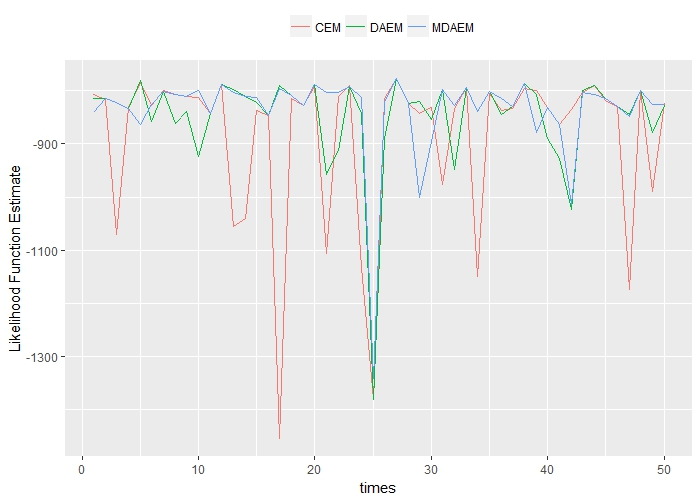
\includegraphics[width=100mm,height=50mm]{1.jpg}
		\caption{???????}
	\end{figure}
	
	???4.1????????????????????????????????????????????????????????????????
	
	\begin{center}
		\begin{table}[htb]
			\linespread{1.5}
			\begin{center}
				\caption{?????????????}
				\small{\begin{tabular}{ccccccccc}
						\hline ?? & ?? & ??? & ??? & ??? & ??? & ?? & ?? & JB??? \\
						\hline  800 &  -0.0002 &  -0.0001 & 0.0544 & -0.0786 & 0.0139 &  -0.5569 & 4.0400 & 590.3197(0)\\
						\hline
				\end{tabular}}
				\label{tab:size}
			\end{center}
		\end{table}
	\end{center}
	
	???4.4?????????????????????????????????0??????????????????????3?????????????????JB?????????p???? 0????????????
	
	??ADF??????????????????????DF??-8.632?$p$??0.01???????0.05???????????????????
	
	???????Hill???$\hat{\alpha}_{r}(k)$???$\left\{r_t\right\}$??????$$\hat{\alpha}_{r}(k)=\left\{\frac{1}{k} \sum_{i=1}^{k} \log \left(\frac{r_{(i)}}{r_{(k+1)}}\right)\right\}^{-1},$$
	??$\left\{r_{(t)}\right\}_{t=1}^{n}$??$\left\{r_{t}\right\}_{t=1}^{n}$???????$\left\{\hat{\alpha}_{r}(k)\right\}_{k=10}^{200}$?????4.2??????????$r_t$??????????1?2?????????$E r_{t}^{2}=\infty$??????????(\ref{204})???SM-???????
	
	\begin{figure}[htb]
		\centering
		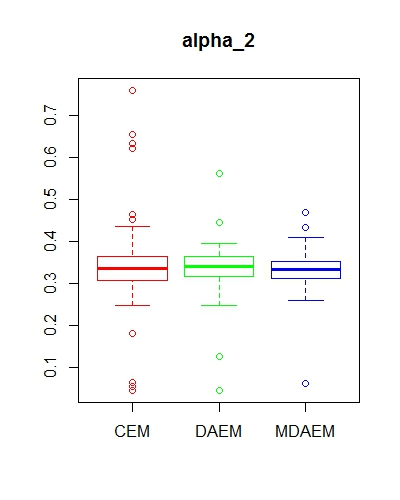
\includegraphics[width=120mm,height=50mm]{4.jpg}
		\caption{????Hill?}
	\end{figure}
	
	??ARMA?????????????ARMA?????????ACF??PACF???????????
	\begin{figure}[htb]
		\centering
		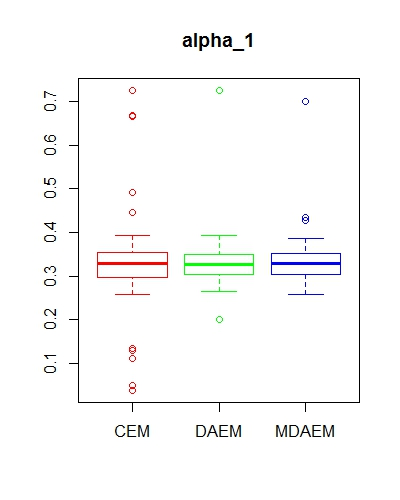
\includegraphics[width=140mm]{3.eps}
		\caption{????ACF??PACF?}
	\end{figure}
	
	?4.3?????10???????????3????????3????????????2???????ACF???20??23??PACF???14???2??????????????????????????????????????????????~ARMA~(0,1)?~ARMA~(0,2)?~ARMA~(0,3)?~ARMA~(1,0)?~ARMA~(1,1)?~ARMA~(1,2)?~ARMA~(1,3)?~ARMA~(2,0)?~ARMA~(2,1)?~ARMA~(2,2)?~ARMA~(2,3)?~ARMA~(3,0)?~ARMA~(3,1)?~ARMA~(3,2)?~ARMA~
	(3,3)?????(\ref{202})??AIC????????????ARMA$(p,q)$???????LS???LAD???SLAD???S-Huber???????ARMA ????????ARMA(2,1)???
	
	?????????????~ARMA~(2,1)?????????Box-Ljung??????????????????????4.5?????p???????????????????ARMA(2,1) ????????????
	\begin{center}
		\begin{table}[htbp]
			\begin{center}
				\caption{Box-Ljung??}
				\small{\begin{tabular}{ccccc}
						\hline    &   LS  &  LAD  & SLAD & S-Huber \\
						\hline Q(6) & 3.1792 & 4.9676 & 4.9276 & 3.6344 \\
						\hline p-value   & 0.786 & 0.548 & 0.5531 & 0.726   \\
						\hline Q(12) & 8.1198 & 10.3 & 10.302 & 8.8337 \\
						\hline p-value   & 0.7757 & 0.5897 & 0.5895 & 0.7171 \\
						\hline
				\end{tabular}}
				\label{tab:size}
			\end{center}
		\end{table}
	\end{center}
	
	?????4.4??QQ???????????????????????
	\newpage
	\begin{figure}[htb]
		\centering
		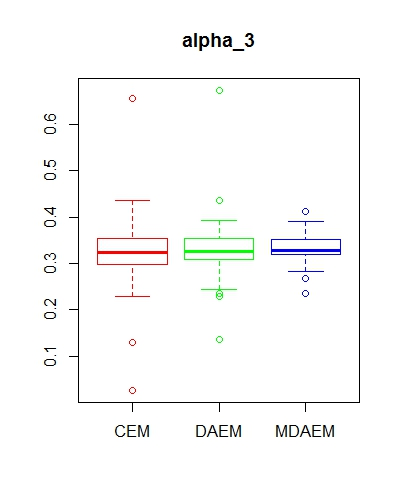
\includegraphics[width=100mm]{5.eps}
		\caption{??QQ?}
	\end{figure}
	
	????????R???ArchTest?????ARMA?????????6?12????????????4.6?????????$p$??????????????ARMA ?????????????
	\begin{center}
		\begin{table}[htb]
			\begin{center}
				\caption{ArchTest??}
				\small{\begin{tabular}{ccccc}
						\hline    &   LS  &  LAD  & SLAD & S-Huber \\
						\hline $\chi^2(6)$ & 27.473 & 27.916 & 27.92 & 28.397 \\
						\hline p-value   & 1.18e-04 & 9.74e-05 & 9.73e-05 & 7.91e-05 \\
						\hline $\chi^2(12)$ & 28.231 & 29.797 & 29.836 & 29.777 \\
						\hline p-value   & 5.12e-03 & 3.00e-03 & 2.96e-03 & 3.02e-03 \\
						\hline
				\end{tabular}}
				\label{tab:size}
			\end{center}
		\end{table}
	\end{center}
	
	??????????ARMA(2,1)????????????????????????????????$t$???GARCH(1,1) ????????GARCH(1,1)???????????????????????????????????ARMA(2,1)-GARCH(1,1)????800??????????????????????(MSE)???????(MAE)?????4.7?
	\begin{center}
		\begin{table}[htb]
			\begin{center}
				\caption{???????????}
				\small{\begin{tabular}{ccccc}
						\hline    &   LS  &  LAD  & SLAD & S-Huber \\
						\hline MSE & 0.000442 & 0.000399 & 0.000379 & 0.000368 \\
						\hline MAE & 0.015286 & 0.014525 & 0.014151 & 0.013932 \\
						\hline
				\end{tabular}}
				\label{tab:size}
			\end{center}
		\end{table}
	\end{center}
	
	\newpage
	??????????S-Huber?????ARMA(2,1)-GARCH(1,1)??????????LS?????MSE???16.73\%?MAE???8.85\%??LAD?????MSE ???7.71\%?MAE???4.08\%???SLAD????????????????SM-???????????????S-Huber??????????ARMA(2,1)-GARCH(1,1)????
	$$
	\left\{\begin{array}{l}{r_{t}=-0.7406r_{t-1}-0.0586r_{t-2}+\varepsilon_t+0.7336\varepsilon_t} \\ {\varepsilon_{t}=\eta_{t} h_{t}} \\ {h_{t}^{2}=0.0552\varepsilon_{t-1}^{2}+0.9386 h_{t-1}^{2}}\end{array},\right.
	$$
	???????????
	
	\chapter[?????]{?????}
	\section{??}
	
	?Box?Jenkins(1970)??????ARMA??????????????????????????????????????????????????????LS???LAD??????????????????????????????????????????????LS??????????LAD ???????????????????????????SM-???????????????????????????
	
	?1????ARMA???????????????????LS???LAD???SM-????????????ARMA???SM-???????????ARMA???SM-???
	
	?2?????????????ARMA????????????????????????????SM-?????????????
	
	?3??????????????????SM-???LAD???LS?????????????????????????????????????????????????SM-??????????
	
	?4?????????????????SM-???LAD????LS???????ARMA??????????GARCH??????????SM-??????????????????
	
	\section{??}
	
	?1???????ARMA???SM-?????????????????????????????????????????????????????????????SM-??????
	
	?2????SM-?????????????SLAD???S-Huber???????????SM-????????????$\rho(\cdot)$????Hampel ???????????????????????????SM- ?????????
	
	?3???????????????????????????????SM-?????ARMA?????????????
	
	
	
	\bibliography{bibliography}
	
	%%%%%%%%%%%%%%%%%%%%%%%%%%%%%%%%%%%%%%%%%%%%%%%%%%%%%%%%%%%????
	\newpage
	\pagestyle{fancy}
	\begin{spacing}{1.2}
		\begin{thebibliography}{99}\wuhao{
				\bibitem{1} ??, ???. ??ARMA???????????????[J]. ????????, 2011, 41(22):84-90.
				\bibitem{1} ???, ???. ????????GDP???????????ARMA???????[J]. ?????????(?????), 2011, 12(2):105-108.
				\bibitem{1} ??,???. ??ARMA-GARCH?????300??????????[J]. ????,2018, (6):44-46.
				\bibitem{1} ???, ??, ??. ?? ACD ??? M ??[J]. ??????, 2014, 37(5):926-945.
				\bibitem{1} ??, ??. ?????????ARMA-GARCH?????[J]. ????????, 2010, 33(7):1108-1112.
				\bibitem{1} ???, ???, ???. ??GARCH?????????????[J]. ????????, 2003, 33(11):65-71.
				\bibitem{1} ???, ???, ???,???. ??ARMA-GARCH???????????[J]. ??, 2006, 31(1):5-8.
				\bibitem{1} ???, ??, ??. ?????????ARMA-GARCH???????????[J]. ??????, 2011, 21(3):16-21.
				\bibitem{1} ???. ???2006~2013????????ARIMA?????[D]. ??:????, 2015:20-26.
				\bibitem{1} ??. ARMA-GARCH???????????????????[J]. ?????, 2006, 15(5):128-132.
				\bibitem{1} ??. ?? ARMA-GARCH ?????????????[J]. ????????(????), 2012, 26(10):36-39.
				\bibitem{1} ???. ????GARCH??????[J]. ??????????, 2006, 16(5):45-49.
				\bibitem{1} ???.???????GARCH????????[J].??????????, 2001, (6):126-129.
				\bibitem{1} ???. ??????????????[J]. ???????, 1999, 20(4): 80-87.
				\bibitem{1} ???, ???, ???. ??????????????ARCH??[J]. ????, 1997, 15(1):43-46.
				\bibitem{1} An H Z, Chen Z G. On convergence of LAD estimates in autoregression with infinite variance[J]. Journal of Multivariate Analysis, 1982, 12(3):335-345.
				\bibitem{1} Anggraeni W, Vinartir R A, Kurniawati Y D. Performance comparisons between ARIMA and ARIMAX method in moslem kids clothes demand forecasting: case study[J]. Procedia Computer Science, 2015, 72:630-637.
				\bibitem{1} Bollerslev T. Generalized autoregressive conditional heteroslcedasticity[J]. Journal of Econometrics, 1986, 31(3):307-327.
				\bibitem{1} Box G E P, Jenkins G M. Time series analysis: forecasting and control[M]. ~San ~Francisco, ~California:Holden Day, 1970.
				\bibitem{1} Box G E P, Jenkins G M, Reinsel G C. Time series analysis: forecasting and control[M]. Englewood Cliffs, New Jersey: Prentice-Hall, 1994.
				\bibitem{1} Chow Y S, Teicher H. Probability theory: independence, interchangeability, Martingales[M]. New York and Heidelberg: Springer-Verlag, 1978.
				\bibitem{1} Davis R A. Gauss-Newton and M-estimation for ARMA processes with infinite variance[J]. Stochastic Processes and Their Applications, 1996, 63:75?95.
				\bibitem{1} Davis R A, Knight K, Liu J. M-estimation for autoregressions with infinite variance[J]. Stochastic Processes \& Their Applications, 1992, 40(1):145-180.
				\bibitem{1} Ding Z, Granger C W J, Engle R F. A long memory property of stock market returns and a new model[J]. Journal of Empirical Finance, 1993, 1(1):83-106.
				\bibitem{1} Durrett R. Probability: Theory and Examples[M]. Thomson-Brooks/Cole, 2005.
				\bibitem{1} Engle R F. Autoregressive conditional heteroscedasticity with estimates of the variance of United Kingdom inflation[J]. Econometrica, 1982, 50(4):987-1007.
				\bibitem{1} Engle R F, Lilien D M, Robins R P. Autoregressive conditional heteroskedasticity with estimates of the variance of UK inflation[J]. Econometrica, 1987, 55(2):391-407.
				\bibitem{1} Glosten L R, Jagannathan R, Runkle D E. On the relation between the expected value and the volatility of the nominal excess return on stocks[J]. The Journal of Finance, 1993, 48:1779-1801.
				\bibitem{1} Gross S, Steiger W L. Least absolute deviation estimates in autoregression with infinite variance[J]. Journal of Applied Probability, 1979, 16(1):104-116.
				\bibitem{1} Hannan E J, Kanter M. Autoregressive processes with infinite variance[J]. Journal of Applied Probability, 1977, 14(2):411-415.
				\bibitem{1}  Huber P J. Robust Regression: Asymptotics, conjectures and Monte Carlo[J]. Annals of Statistics, 1973, 1(5):799-821.
				\bibitem{1} Insel A, Karaka M, Sualp M N. A comparative analysis of the ARMA and neural networks models. A case of Turkish economy[J]. Iktisat Isletme ve Finans, 2010, 25(290):35-64.
				\bibitem{1} Kanter M, Steiger W L. Regression and autoregression with infinite variance[J]. Advances in Applied Probability, 1974, 6(4):768-783.
				\bibitem{1} Kolmogoroff A N. $\ddot{\mathrm{U}}$ber das gesetz des iterierten Logarithmus[J]. Mathematische Annalen, 1929, 101:126-135.
				\bibitem{1} Ling S. Self-weighted least absolute deviation estimation for infinite variance autoregressive models[J]. Journal of the Royal Statistical Society, 2005, 67(3):381?393.
				\bibitem{1} Ling S. Self-weighted and local quasi-maximum likelihood estimators for ARMAGARCH/IGARCH models[J]. Journal of Econometrics, 2007, 140(2):849-873.
				\bibitem{1} Ling S, McAleer M. Asymptotic theory for a new vector ARMA-GARCH model[J]. Econometric Theory, 2003, 19:280-310.
				\bibitem{1} Ling S, McAleer M. A general asymptotic theory for time-series models[J]. Statistica Neerlandica, 2010, 64:97-111.
				\bibitem{1} Mikosch T, Gadrich T, Adler R J. Parameter estimation for ARMA models with infinite variance innovation[J]. Annals of Statistics, 1995, 23(1):305-326.
				\bibitem{1} Nelson D B. Conditional, heteroscedasticity in asset returns: a new approach[J]. Econometrics, 1991, 59:347-370.
				\bibitem{1} Pan J, Wang H, Yao Q. Weighted least absolute deviations estimation for ARMA models with infinite variance[J]. Econometric Theory, 2007, 23(5):852-879.
				\bibitem{1} Pollard D. New ways to prove central limit theorems[J]. Econometric Theory, 1985, 1:295?314.
				\bibitem{1} Tang H, Chiu K C, Xu L. Finite mixture of ARMA-GRACH model for stock price prediction[C]. North Carolina: Proc. of 3rd International Workshop on Computational Intelligence in Economics and Finance, 2003:1112-1119.
				\bibitem{1} Walker G. On periodicity in series of related terms[J]. Proceedings of the Royal Society of London, Series A, 1931, 131(818):518-532.
				\bibitem{1} Wang X, Hu S. Asymptotics of self-weighted M-estimators for autoregressive models[J]. Metrika, 2017, 80:1-10.
				\bibitem{1} Williams B. Multivariate vehicular traffic flow prediction: evaluation of  ARIMAX modeling[J]. Transportation Research Record Journal of the Transportation Research Board, 2001, 1776(1):194-200.
				\bibitem{1} Yule G U. On a method of investigating periodicities in disturbed series in spectral reference to wolfer's son spot numbers[J]. Philosophical Transactions of the Royal Society, Series A, 1927, 226:267-298.
				\bibitem{1} Zhu K. and Ling S. Global self-weighted and local quasi-maximum exponential likelihood estimators for ARMA-GARCH/IGARCH models[J]. Annals of Statistics, 2011, 39:2131- 2163.
				\bibitem{1} Zhu K, Ling S. LADE-based inference for ARMA models with unspecified and heavy-tailed heteroscedastic noises[J]. Journal of the American Statistical Association, 2015, 110(510):784-794.}
		\end{thebibliography}
	\end{spacing}
	
	?
	\addcontentsline{toc}{chapter}{????}
	
	
	
	
	
	
	
	%%%%%%%%%%%%%%%%%%%%%%%%%%%%%%%%%%%%%%%%%%%%%%%%%%%%%%%%%%%????
	
	
	
	%%%%%%%%%%%%%%%%%%%%%%%%%%%%%%%%%%%%%%%%%%%%%%%%%%%%%%%%%%%%%%%
	%\newpage
	%\pagestyle{fancy}
	%\begin{center}
	%\heiti\sanhao {?\quad ?}
	%\end{center}
	
	%\addcontentsline{toc}{chapter}{??}
	
	
	%%%%%%%%%%%%%%%%%%%%%%%%%%%%%%%%%%%%%%%%%%%%%%%
	%\newpage
	%\thispagestyle{empty}
	%\begin{center}\heiti\sanhao\textbf{?\ ?\ ?\ ?\ ?}\end{center}
	%\begin{spacing}{2.0}
	%????????????????????????????????????.????,?????????????????,??????????????????????,???????????????????????????????????.??????????????????????????????????????.\\
	%
	%~~~~~~~~~~~~~~~~~~??:\underline{\hspace{3cm} }\ \ ??: \hspace{0.8cm} ? \hspace{0.2cm} ? \hspace{0.4cm} ?\\
	%%~~~~~~~~~~~~~~~~~~??:\underline{\hspace{0.8cm} ??? \hspace{0.8cm}}\ \ ??: 2018 ? 1 ? 14 ?\\
	%\\
	%
	%\begin{center}\heiti\sanhao\textbf{ ???????????}\end{center}
	%~~~~~~????????????????????????????????????????????????????????????????,??????????,??????????????????????????,??????????????????????????,??????????????????????.
	%
	%?????????????????.\\
	%
	%~~~~~~~~~~~~~~~~~~??:\underline{\hspace{3cm} }\ \ ????:\underline{\hspace{3cm}}
	%%~~~~~~~~~~~~~~~~~~??:\underline{\hspace{0.8cm} ??? \hspace{0.8cm}}\ \ ????:\underline{\hspace{0.8cm} ??? \hspace{0.8cm}}
	%
	%~~~~~~~~~~~~~~~~~~~~~~~~~~~~~~~~~~~~~~~~~~~~~~~~~~~ ??: \hspace{0.8cm} ? \hspace{0.2cm} ? \hspace{0.4cm} ?
	%%~~~~~~~~~~~~~~~~~~~~~~~~~~~~~~~~~~~~~~~~~~~~~~~~~~~ ??: 2018 ? 1 ? 14 ?
	%\end{spacing}
	%%%%%%%%%%%%%%%%%%%%%%%%%%%%%%%%%%%%%%%%%%%%%%%%%%%%%%%%%%%%%%%%%%%%%%%%%%%%%
	
	
\end{document}

